\section{Planning}%
\label{sec:planning}
This section explains \textit{path planning}, which consists of 2 steps. Firstly, path estimation, and secondly, motion or manipulation planning. The path estimator can detect non-existent paths and concludes such paths as unfeasible~\cite{zhang_simple_2008}. If a path exists, the double tree \ac{RRT*} planning algorithm is responsible for finding a path from starting point to a target point in configuration space whilst respecting applicable constraints~\cite{chen_fast_2018}.\bs

\todo{So how are the nonholonomic constraints checked? Eleborate en become clear about that? f}
To clarify terminology used in this thesis, the following \Cref{table:termology_planning} is presented.\bs
\noindent
\begin{table}[H]
  \centering
  \begin{tabular}%
  {>{\raggedright\arraybackslash}p{0.25\textwidth}%
   >{\raggedright\arraybackslash}p{0.65\textwidth}}
  Global Planning:& Planning for a task by focusing on one single subtask at a time. \\
  Local Planning:& Validating if two closeby configurations that are maximal \textit{step\_size} apart can be connected whilst respecting constraints using a system model.\\
  Path Estimation:& Estimating the existence of a path for a push or drive action.\\
  Motion Planning:& Planning a drive action\\
  Manipulation Planning:& Planning for an push action.\\
  Action Planning:& Planning for an drive or push action.\\
  Path Planning:& Path estimation and action planning for an drive or push action.\\
  \end{tabular}
\caption{The planning-related terminology is juxtaposed in the left column\\alongside its corresponding description in the right column.}%
\label{table:termology_planning}
\end{table}

\subsection{Estimating Path Existence}%
\label{subsec:path_estimation}
In this subsection, motivation and explanation for estimating path existence are presented. We can describe the path estimation algorithm as \textit{The idea is to discretize the configuration space. The emerging cells act as nodes in the graph, cells connect through edges to nearby cells. Graph-based planners start from the cell containing the starting configuration and search for the cell containing the target configuration while avoiding cells in obstacle space.\bs}

If the path estimator concludes the existence of a path planning problem, then it is validated that it is geometrically possible for an object to go from start to target configuration in small successive steps without colliding with an unmovable obstacle. The check prevents the planner from attempting a search for a start and target configuration for a problem that is unfeasible due to not being detected by the path estimator because it does not check for nonholonomic constraints. By neglecting nonholonomic constraints, the path estimator is magnitudes faster than the planner; the planner is responsible for checking the nonholonomic constraints.

\paragraph{Discritizing the Configuration Space}
For general geometric shapes, a configuration space can be constructed and discretized. During this thesis, configuration space was implemented for cylinders and rectangular prisms. First, the configuration space for a cylindrical-shaped object in a 3-dimensional environment is presented. That configuration space for cylindrical objects is defined as a $(x, y)$-plane, and the $z$-axis is omitted. During the projection from a 3-dimensional environment to a 2-dimensional plane, cylinders (flat side facing down) become circles, and rectangular prisms become rectangles. The definition of configuration space is presented below for a circular object, such as the point robot, without loss of generality. In this thesis, three dimensional objects can be projected to the xy-plane. As a result a three dimensional spherical robot or object can has a configuration space that is two dimensional (\gls{x} and \gls{y} dimension). Objects in the shape of rectangular prisms that are projected onto the xy-plane become rectangles, and have a three dimensional configuration space (\gls{x}, \gls{y} and \gls{theta} dimension).\bs
\bs

A grid of cells represents configuration space. Let \gls{cellSize} be the width and height of a square cell. Let \gls{xGridLength} be the vertical (north to south) length and let \gls{yGridLength} be the horizontal length (west to east) of the configuration space, point $(0, 0)$ is at the center of the grid.\bs

The configuration space for a circular object is defined as:\bs
\[ \gls{cspace}^{\textrm{circle}} =
\begin{bmatrix}
  c_{(0,0)} & c_{(0,1)} & \hdots & c_{(0,j_{\textrm{max}})}\\
  c_{(1,0)} & c_{(1,1)} & \hdots & c_{(1,j_{\textrm{max}})}\\
  \vdots &  \vdots & \ddots & \vdots\\
  c_{(i_{\textrm{max}},0)} & c_{(i_{\textrm{max}},1)} & \hdots & c_{(i_{\textrm{max}},j_{\textrm{max}})}\\
\end{bmatrix}
\]


With $0 \leq i \leq i_{\textrm{max}} = \frac{\gls{xGridLength}}{\gls{cellSize}}, \quad 0 \leq j < j_{\textrm{max}} = \frac{\gls{yGridLength}}{\gls{cellSize}}$.\bs

Where $c_{(i,j)}$ in matrix \gls{cspace} represents to which subspace the cell at indices $(i, j)$ belongs. The four subspaces considered in this thesis are free-, unmovable-, movable- and unknown space indicated with the integers 0, 1, 2 and 3, respectively. Multiple subspaces can reside in a single cell; by default, a cell represents free space. The subspaces are ordered from least to most important: free, movable, unknown, and unmovable space. A cell displays the subspace with the highest order of importance that resides in the cell. Thus a cell that contains part unknown and part unmovable space will evaluate as unmovable space since unmovable space is more important than the unknown space.\bs

A mapping function $f_\mathit{chart\_to\_idx}(i,j)$ maps the\\Cartesian $(x,y)$ coordinates to their associated $(i,j)$ indices:

\[f_\mathit{chart\_to\_idx}(i,j): \gls{R}^2 \mapsto \gls{Rnonnegative}^2 \]

Defined for:
\[\gls{x} = \{\gls{xGridLength} \in \gls{R}: -\frac{\gls{xGridLength}}{2} \leq \gls{x} \leq \frac{\gls{xGridLength}}{2}\},\quad \gls{y} = \{\gls{yGridLength} \in \gls{R}: -\frac{\gls{yGridLength}}{2} \leq \gls{y} \leq \frac{\gls{yGridLength}}{2}\}\]


A mapping function $f_\mathit{idx\_to\_chart}(i, j)$ maps the\\indices $(i, j)$ to their associated Cartesian $(x,y)$ coordinates:
\[f_\mathit{chart\_to\_idx}(i,j): \gls{Rnonnegative}^2  \mapsto \gls{R}^2 \]

Defined for:
\[i = \{\frac{\gls{xGridLength}}{\gls{cellSize}} \in \gls{Rnonnegative}: 0 \leq i \leq \frac{\gls{xGridLength}}{\gls{cellSize}},\quad j = \{\frac{\gls{yGridLength}}{\gls{cellSize}} \in \gls{Rnonnegative}: 0 \leq j \leq \frac{\gls{yGridLength}}{\gls{cellSize}}\}\]


The configuration space for a rectangular object is defined as:\bs

\begin{center}
  \begin{tikzpicture}[every node/.style={anchor=north east,fill=white,minimum width=1.4cm,minimum height=7mm}]
    \node (mA)
      {$\begin{bmatrix}
          c_{(0,0,k_{\textrm{max}})} & c_{(0,1,k_{\textrm{max}})} & \hdots & c_{(0,j_{\textrm{max}},k_{\textrm{max}}))}\\
          c_{(1,0,k_{\textrm{max}}))} & c_{(1,1,k_{\textrm{max}}))} & \hdots & c_{(1,j_{\textrm{max}},k_{\textrm{max}}))}\\
          \vdots &  \vdots & \ddots & \vdots\\
          c_{(i_{\textrm{max}},0,k_{\textrm{max}}))} & c_{(i_{\textrm{max}},1,k_{\textrm{max}}))} & \hdots & c_{(i_{\textrm{max}},j_{\textrm{max}},k_{\textrm{max}}))}\\
      \end{bmatrix}$};

    \node (mB) at ($(mA.south west)+(2.1,0.65)$)
      {$\begin{bmatrix}
          c_{(0,0,1)} & c_{(0,1,1)} & \hdots & c_{(0,j_{\textrm{max}},1))}\\
          c_{(1,0,1))} & c_{(1,1,1))} & \hdots & c_{(1,j_{\textrm{max}},1))}\\
          \vdots &  \vdots & \ddots & \vdots\\
          ttttc_{(i_{\textrm{max}},0,1))} & c_{(i_{\textrm{max}},1,1))} & \hdots & c_{(i_{\textrm{max}},j_{\textrm{max}},1))}\\ % adding character 't' for horizontal spacing
      \end{bmatrix}$};

    \node (mC) at ($(mB.south west)+(1.8,0.8)$)
      {$\begin{bmatrix}
          c_{(0,0,0)} & c_{(0,1,0)} & \hdots & c_{(0,j_{\textrm{max}},0))}\\
          c_{(1,0,0))} & c_{(1,1,0))} & \hdots & c_{(1,j_{\textrm{max}},0))}\\
          \vdots &  \vdots & \ddots & \vdots\\
          c_{(i_{\textrm{max}},0,0))} & c_{(i_{\textrm{max}},1,0))} & \hdots & c_{(i_{\textrm{max}},j_{\textrm{max}},0))}\\
      \end{bmatrix}$};

    \node (Cspace) at ($(mC.south west)+(3,5.7)$)
      {$\gls{cspace}^{\mathit{rectangle}} =$};

    \draw[dashed]([xshift=-0.2cm, yshift=-0.135cm] mA.north east)--([xshift=-0.2cm, yshift=-0.135cm]mC.north east);
    \draw[dashed]([xshift=0.19cm, yshift=-0.135cm] mA.north west)--([xshift=0.19cm, yshift=-0.135cm]mC.north west);
    \draw[dashed]([xshift=-0.2cm, yshift=0.135cm] mA.south east)--([xshift=-0.2cm, yshift=0.135cm]mC.south east);
  \end{tikzpicture}
\end{center}

With $0 \leq i \leq i_{\textrm{max}} = \frac{\gls{xGridLength}}{\gls{cellSize}}, \quad 0 \leq j \leq j_{\textrm{max}} = \frac{\gls{yGridLength}}{\gls{cellSize}}, \quad k \in \gls{Rnonnegative}$.\bs

Similar to $f_\mathit{chart\_to\_idx}(x, y)$ and $f_\mathit{idx\_to\_chart}(i,j)$ the mapping functions $\mathit{chart\_to\_idx}(x, y, \theta)$ and $f_\mathit{idx\_to\_pose}(i, j, k)$ exist and map between the $(x, y, \theta)$ pose and the $(i, j, k)$ indices.\bs

An example configuration space for the point robot is presented below.
\begin{figure}[H]
    \centering
    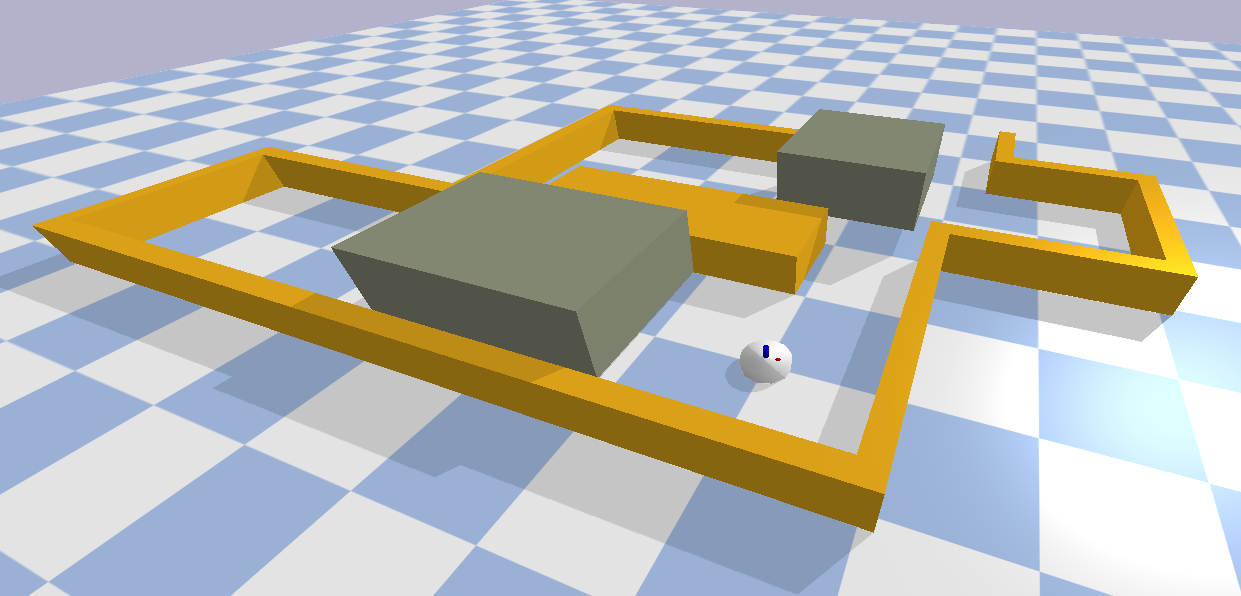
\includegraphics[width=0.9\textwidth]{figures/required_background/planning/two_push_to_freedom_env}
    \caption{Robot environment with the point robot, unmovable yellow walls and movable brown boxes.}%
    \label{fig:two_pushes_to_freedom_env}
\end{figure}

The point robot has a cylindrical shape; thus, a 2-dimensional configuration space is created and can be seen in \Cref{fig:two_pushes_to_freedom_conf_space}.

\begin{figure}[H]
  \centering
  \begin{subfigure}{.49\textwidth}
    \centering
    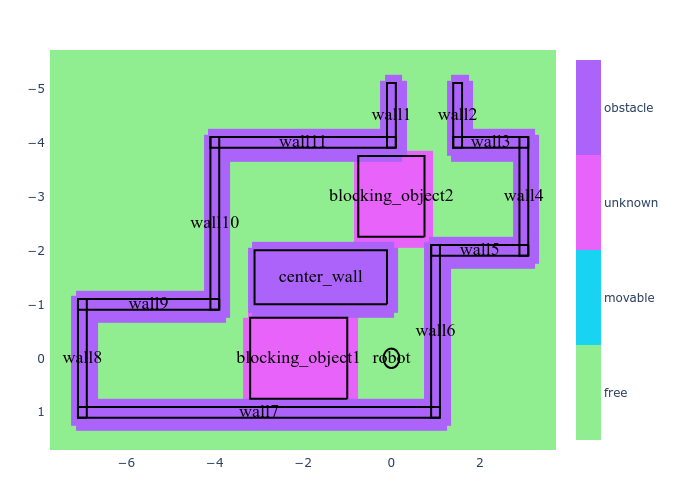
\includegraphics[width=1.05\textwidth]{figures/required_background/planning/c_space_point_robot_grid_size_0_1}
    \caption{$\gls{cspace}^{circle}$ with $\gls{cellSize} = 0.1$}%
    \label{fig:c_space_two_pushes_small}
  \end{subfigure}
  \begin{subfigure}{.49\textwidth}
    \centering
    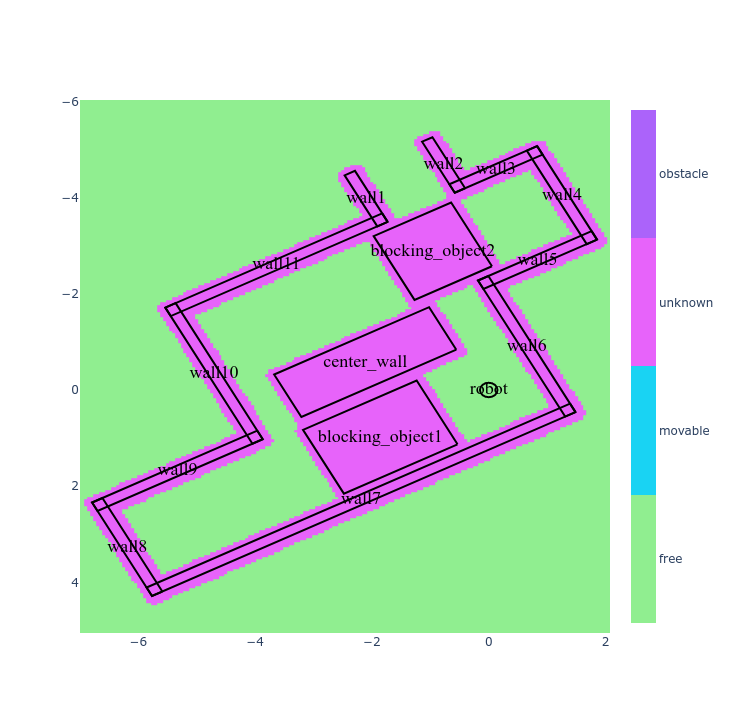
\includegraphics[width=1.05\textwidth]{figures/required_background/planning/c_space_point_robot_grid_size_0_05}
    \caption{$\gls{cspace}^{circle}$ with $\gls{cellSize} = 0.05$}%
    \label{fig:c_space_two_pushes_smaller}
  \end{subfigure}
  \caption{The configuration space for the point robot with different cell sizes. The robot\\environment corresponds to the environment presented in \Cref{fig:two_pushes_to_freedom_env}. The robot classifies\\all objects as unknown since it is unaware of the objects' classes.}
  \label{fig:two_pushes_to_freedom_conf_space}
\end{figure}

The resolution of the configuration space at \Cref{fig:c_space_two_pushes_smaller} is higher compared to \Cref{fig:c_space_two_pushes_small} because of a smaller grid size. A high resolution is better at detecting paths through small corridors and tight corners, but it comes at the cost of a more extended creation and search time.

\paragraph{Path Existence Algorithm} In the context of this thesis, we can describe path existence as: \textit{For an object's discretized configuration space, there exists a list of neighbouring cells from starting to target configuration that does not lie in unmovable space.\bs}

A path in configuration space is detected using the implemented\\$f_\mathit{shortest\_path}(\gls{c}_\mathit{start}, \gls{c}_\mathit{target}, )$ function. This function takes a start- and target configuration, $\gls{c}_\mathit{start}$ and $\gls{c}_\mathit{target}$ and returns the shortest path between them that lies in free space. The \textit{shortest\_path} function searches for the shortest path using the Dijkstra algorithm~\cite{dijkstra_note_1959} on the discreted configuration space. The shortest path validates the existence of a path (note that only geometric constraints are respected), and can help path planning discussed in \Cref{sec:planning}. The shortest path helps path planning by providing an initial number of path planner nodes before the path planner creates nodes by random sampling. Such a conversion is also referred to as a \quotes{warm start}. If no path can be found, the $f_\textit{shortest\_path}$ function raises an error that will prevent path planning from occurring.\bs

\paragraph{Unfeasible solutions and an undecidable problem}
The path estimator does not take system constraints into account. Thus, the path estimator can find a list of neighbouring cells from the start to the target configuration and conclude that a path exists. In reality, this path is unfeasible. An example is driving the boxer robot displayed in \Cref{subfig:example_boxer_robot} through a narrow, sharp corner. Whilst geometrically, the robot would fit through the corner, the nonholonomic constraints of the robot prevent it from steering through such a tight corner. It is for the action planner to detect that the path is unfeasible.\\

The path estimator suffers from another drawback, finding proof that there exists a path that is undecidable~\cite{zhang_simple_2008}. This is due to the chosen cell size during discretizing the configuration space. An example is a corridor having the same width as the robot. The robot fits exactly through this corridor. Detecting such a path requires many neighbouring cells that lie exactly in the center line of the corridor. Only with a cell size going to zero and the number of cells going to infinity such a path is guaranteed to be detected. Path non-existence, on the other hand, is easier to prove because the path estimator provides an upper bound on existing paths and a lower bound on non-existing paths~\cite{zhang_simple_2008}. The following flowchart neatly presents why the existence of paths is an \textit{estimation} rather than an guarantee.\bs

\begin{figure}[H]
\centering
\begin{tikzpicture}]

    % Nodes
    \node [decision, text width=8em, line width=1pt] (first) { Can the path estimator find a path between start- and target configuration? };

    \node [block, below left=1cm and 1cm of first, minimum width=13em, text width=12em, line width=1pt] (path_exists) { A path does exist, however,it can still be unfeasible due to constraints other than the geometric constraints };
    \node [block, below right=1cm and 1cm of first, minimum width=13em, text width=12em, line width=1pt] (path_does_not_exists) { A path could not be found, however, due to the \textit{finite} discretization a path could exist and could not be found};

    \draw[>=stealth, ->, line width=1.0pt] (first.west) [out=180, in=90] to node[xshift=-0.3cm, above] {\large yes} (path_exists.north);
    \draw[>=stealth, ->, line width=1.0pt] (first.east) [out=0, in=90] to node[xshift=0.3cm, above] {\large no} (path_does_not_exists.north);

\end{tikzpicture}
% \vspace{-5cm}
\caption{Flowchart displaying both drawbacks when checking path existence. These drawbacks\\motivate why the existence of a path can only be \textit{estimated} rather than guaranteed.}%
\label{tikz:flowchart_path_estimator}%
\end{figure}

The path existence algorithm can detect non-existence paths. Thus checking path existence before motion or manipulation planning filters out several non-existent paths saving time and resources. Even if, in exceptional cases, the path estimator can yield unfeasible paths and fails to detect existing paths. Checking path existence before path planning filters some non-exist paths and is additionally motivated by two reasons. First, path estimation is orders of magnitude faster compared to path planning. Secondly, the path estimation algorithm can provide a number of initial nodes to the path planner that can act as a \quotes{warm start}.


\subsection{Motion Planning}%
\label{subsec:motion_planning}
Controllers discussed in \Cref{sec:control_methods} can track a path from start to target, given that all necessary ingredients are provided. One essential ingredient is a path to follow, and providing a path is the planners' responsibility; planners seek inside the configuration space for a path from the start to the target configuration. A practical example of such a path is a list of successive points in configurations space. How far the successive points can lie apart is a tuning parameter of the planner. Seeking a path in configuration space whilst avoiding unmovable objects is referred to as \textit{path planning} and can be described as:\bs

\textit{\quotes{The main idea is to avoid the explicit construction of the object space and instead conduct a search that probes the configuration space with a sampling scheme. This probing is enabled by a collision detection module, which the path planning algorithm considers a “black box.”~\cite{lavalle_planning_2006}}}\bs

The path planner is defined with the following tuple:

\[\mathit{Path Planner} = \left\langle \gls{nodesMP}, \gls{edgesMP}, \gls{pathsMP}\right\rangle\]

Where \gls{nodesMP} is a set of nodes, \gls{edgesMP} a set of edges and \gls{pathsMP} a set of paths, a path is defined as:

\[\mathit{path} = [\gls{c}_\mathit{start}, \gls{c}_2, \gls{c}_3, \cdots, \gls{c}_{n-1}, \gls{c}_\mathit{target}]\]

Where $n \in \mathbb{Z}_{\geq 2}$ is the number of configurations in the path.\bs

The goal of the path planner is to find a path between a given start- and target configuration that results in the lowest \textit{TotalPathCost}, defined as:\bs

\[\mathit{TotalPathCost} = \sum_{i=1}^{n-1} \mathit{Distance}(\gls{c}_i, \gls{c}_{i+1}) \sum_{i=1}^{n-1} = \left\|\gls{c}_i-\gls{c}_{i+1}\right\|\]

Now pseudocode of the \ac{RRT*} algorithm is presented that is split into three parts that are grouped by color as can be seen in \Cref{pseudocode:proposed_rrt_star_all}. Notice that the colour correspond to the later pseudocode and example figures. Each part is then discussed, as well as a number of variables and functions used in that respected part. When discussing each part an example is analyzed in which the path planner adds a single node to the connectivity graph. The variables and functions are neatly grouped after discussing the example in \Cref{table:functions_for_proposed_rrt_star}. Note that, the path planner in this section plans in free- and obstacle (or unmovable) space, later in \Cref{chap:proposed_planning} that will be extended to free-, unknown-, movable- and unmovable space.\bs

A node $x$ in the path planner consists of the following tuple:\bs
\[x = \left\langle \gls{c}, \mathit{cost\_to\_source}, \mathit{key}, \mathit{prev\_node\_key}, \mathit{in\_tree} \right\rangle\]

Where \gls{c} is a point in configuration space, \textit{cost\_to\_source} the cost toward the source node, \textit{key} a unique key for the node, \textit{prev\_node\_key} they parent key to which the node is directly connected with an edge, \textit{in\_tree} an indicator that the node is connected to the \textit{start-} or \textit{target} connectivity tree. The path planner starts by adding the first two initial nodes, the start- and target node. The path planner then enters a loop that adds randomly sampled nodes, until the stopping criteria is reached with the \textit{NotReachStop} function.\bs

% ALL
\begin{algorithm}[H]
\caption{Pseudocode for double tree \ac{RRT*} algorithm. The pseudocode is split into three parts, \Cref{pseudocode:proposed_rrt_star_one,pseudocode:proposed_rrt_star_two,pseudocode:proposed_rrt_star_three} that correspond to the blue, yellow and green coloured blocks.}%
\label{pseudocode:proposed_rrt_star_all}%
\begin{algorithmic}[1]

\hspace{-0.9cm}\colorbox{my_grey}{\parbox{\linewidth}{%
\State $\gls{nodesMP} \leftarrow x_{init}$
\While{\textit{NotReachStop}}

\hspace{-0.1cm}\colorbox{my_light_blue}{\parbox{\linewidth}{%
   \algorithmiccomment{Create, project and validate a new random node}
}}

\hspace{-0.1cm}\colorbox{my_yellow}{\parbox{\linewidth}{%
    \algorithmiccomment{Find and connect new node to parent node}
}}

\hspace{-0.1cm}\colorbox{my_green}{\parbox{\linewidth}{%
  \algorithmiccomment{\parbox[t]{.6\linewidth}{Check if the newly added node can lower cost for nearby nodes and if a both connectivity trees can be connected}}
}}
\EndWhile
}}
\end{algorithmic}
\end{algorithm}

The example that adds a single node starts in \Cref{fig:motion_planner_adding_one_node_all}. In this example, one node is added to the starting connectivity tree. Adding this node involves the following steps: generating a new random node, projecting the node to the nearest node, rewiring nearby nodes and connecting the start to the target tree.\bs

The start connectivity tree consists of the nodes connected by edges containing the starting node, and vice versa for the target connectivity tree containing the target node. The algorithm grows the two \textit{connectivity trees} by randomly sampling configurations and adding them as nodes to the start or target connectivity tree. The algorithm explores configuration space by growing these connectivity trees.\bs

\begin{figure}[H]
    \centering
    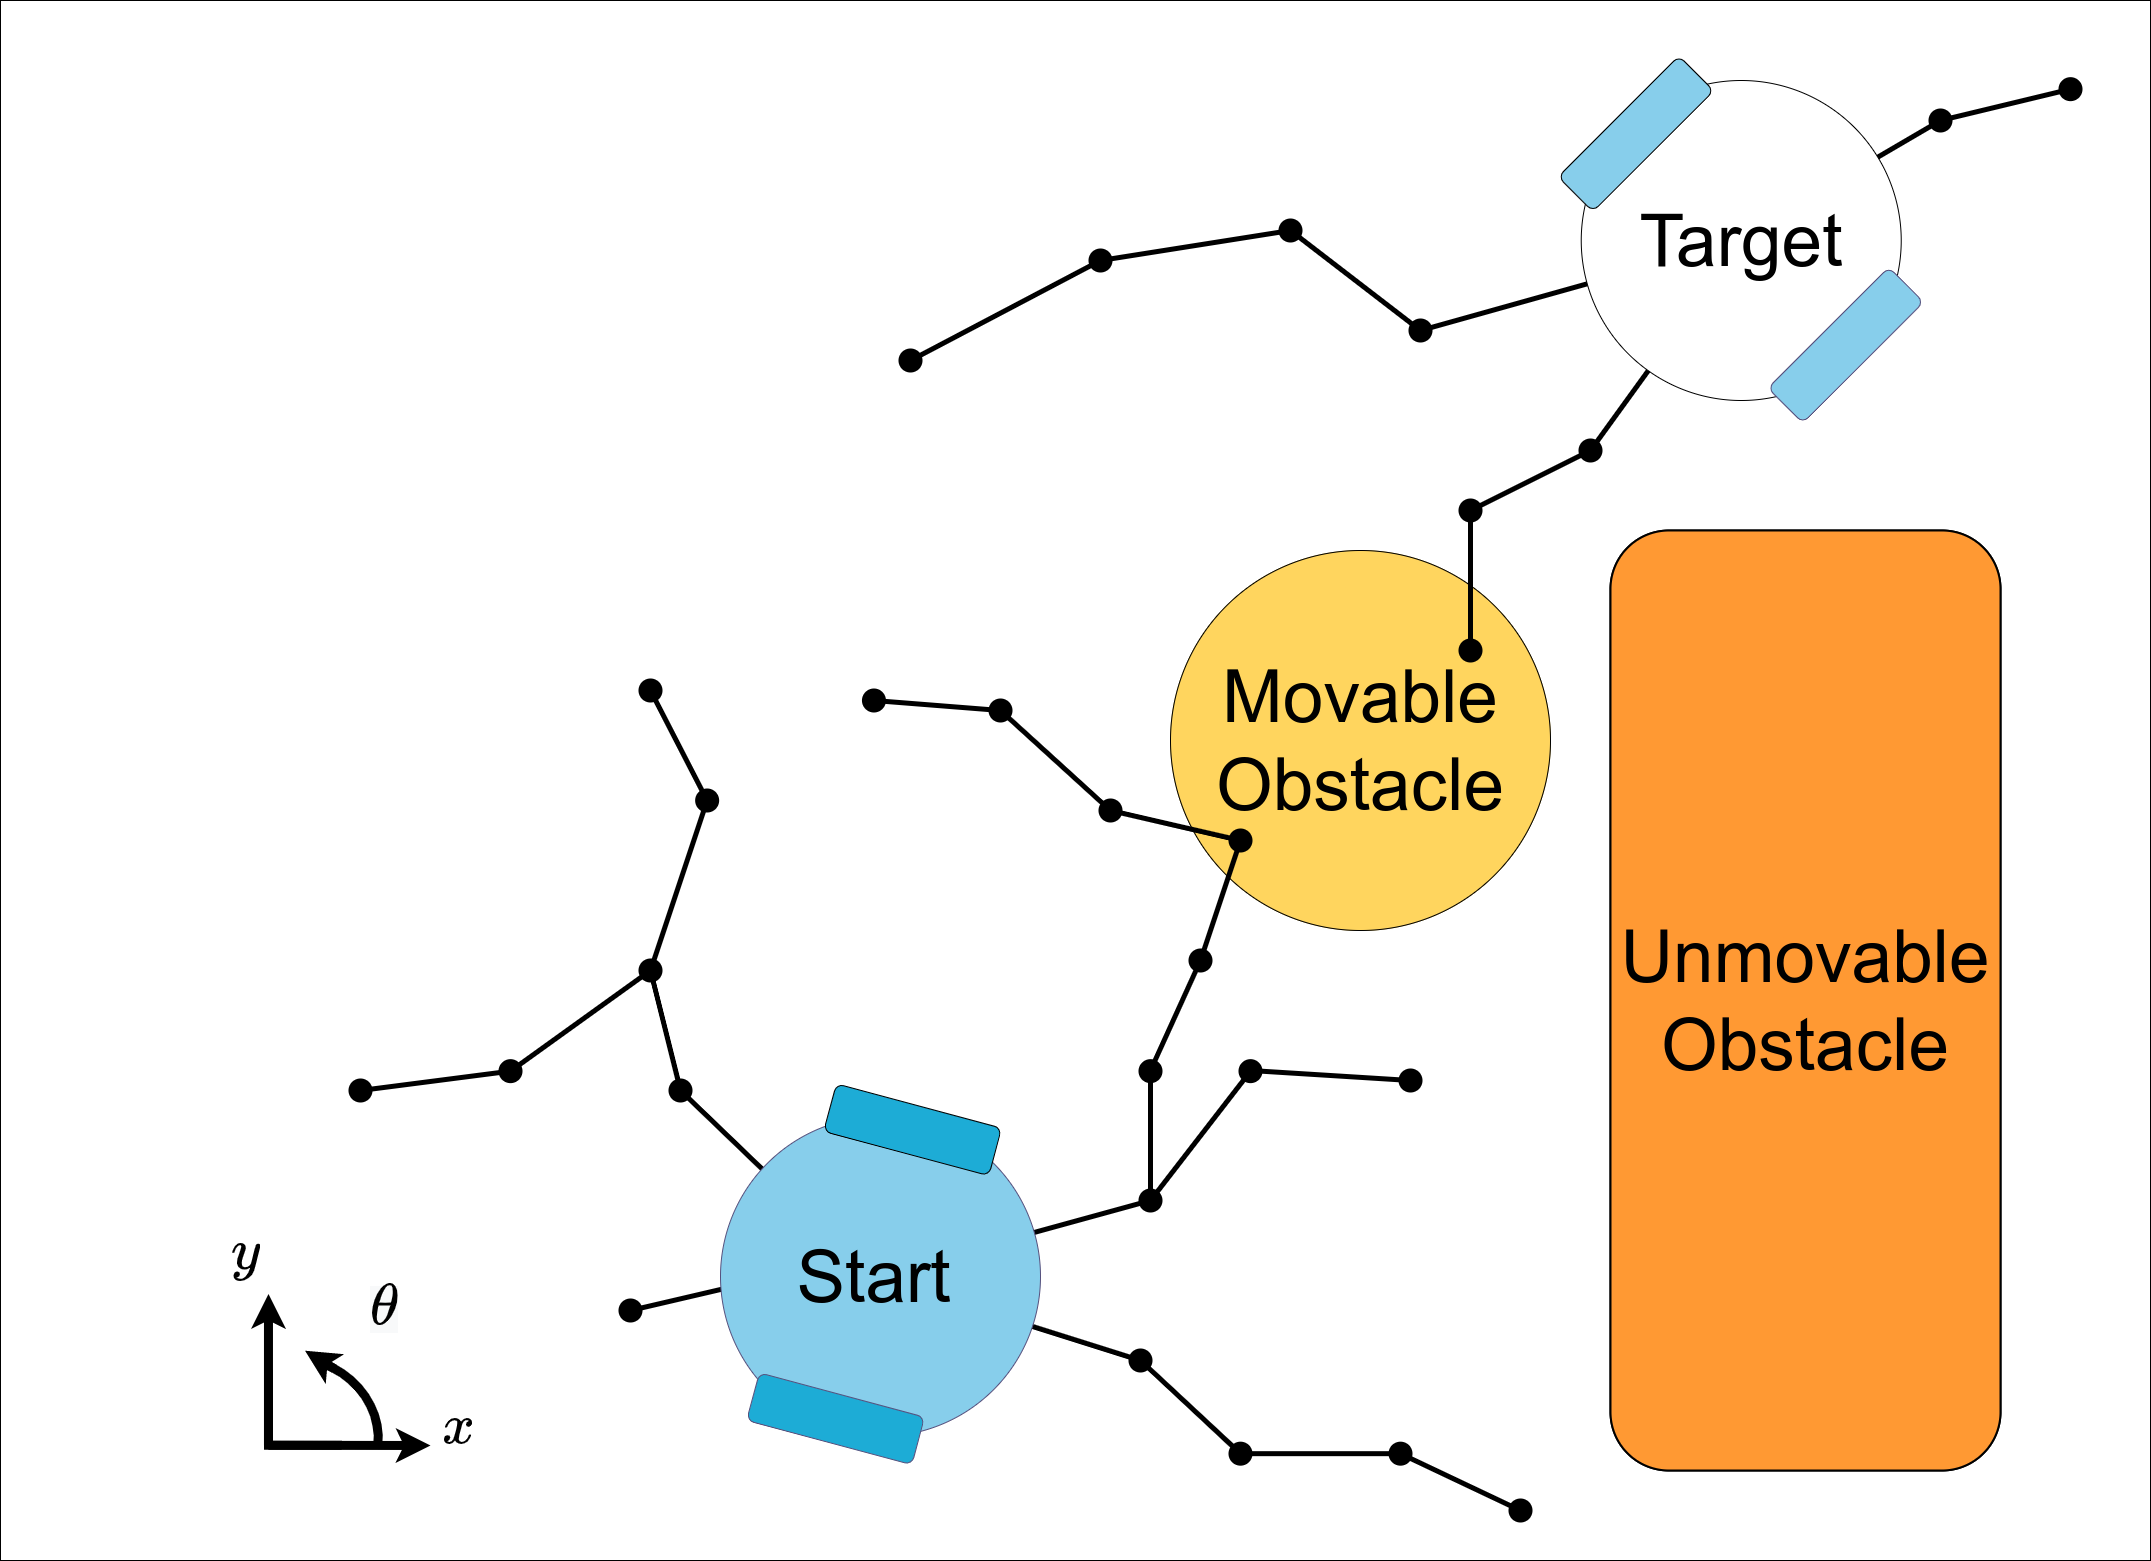
\includegraphics[width=0.5\textwidth, cfbox=my_grey 5pt 0pt]{figures/required_background/mp/1mp_init.drawio.png}
    \caption{Snapshot of a two dimensional configuration with free- and unmovable space. Where unmovable space is indicated by the unmovable object and the rest of the configuration space, including the movable object, is free space. The start- and target nodes, denoted as \quotes{Start} and \quotes{Target} respectively, serve as the source nodes for the start- and target connectivity tree.}
    \label{fig:motion_planner_adding_one_node_all}
\end{figure}

The algorithm has two tuning parameters that can be tweaked; first, the \textit{step size}, the maximal normalized distance between connected nodes in the connectivity trees, see \Cref{subfig:mp_step_size} for a visual example. Choosing a high step size will increase search speed because the connectivity trees grow faster. A higher step size comes at the cost of smoothness; the resulting path will be bumpier with sharper corners. Additionally, the path has an increased chance of collision with unmovable objects because, for two connected configurations in a path, the individual configurations can both lie in free space whilst a direct line between the configurations crosses through unmovable space. The second tuning parameter is the \textit{search size}, which is a subspace around the newly sampled node (see, \Cref{fig:motion_planner_adding_one_node_tree}).\bs

% ONE
\begin{algorithm}[H]
\caption{Pseudocode to create, project and validate a new random node.}%
\label{pseudocode:proposed_rrt_star_one}
\begin{algorithmic}[1]
  \hspace{-0.9cm}\colorbox{my_light_blue}{\parbox{\linewidth}{%
    \State $\gls{nodeMP}_\mathit{rand} \leftarrow \mathit{Sample_{random}}$
    \State $\gls{nodeMP}_\mathit{nearest} \leftarrow \mathit{Nearest(\gls{nodeMP}_{rand}, \gls{nodesMP})}$
    \State $\gls{nodeMP}_\mathit{temp} \leftarrow \mathit{Project(\gls{nodeMP}_{rand}, \gls{nodeMP}_{nearest})}$

    \If{$\mathit{CollisionCheck(\gls{nodeMP}_{temp})}$}
    \State $\gls{nodeMP}_\mathit{new} = \gls{nodeMP}_\mathit{temp}$
    \State $Cost_\mathit{toInitMin} \leftarrow +\infty$
    \Else
        \State Continue
    \EndIf
}}
\end{algorithmic}
\end{algorithm}

The $\mathit{Sample_{random}}$ function creates a random node in free- or unmovable space. This random node is projected to the closes existing node using two functions. First, the $\mathit{Nearest}(x, V)$ returns the nearest node from $x$ in $V$. Second, if the nearest node is further than \textit{step size} Euclidean distance from the randomly sampled node, then the $\mathit{Project}(x, x')$ function projects $x$ toward $x'$, such that the Euclidean distance between $x$ and $x'$ is the \textit{step size}. The projected random node can reside in free- or unmovable space, ensuring that the node is in free space is validated with the $\mathit{CollisionCheck}(x)$ function that returns true if $x$ is in free space. Newly sampled nodes are added structurally, guaranteeing an optimal path is found with infinite sampling~\cite{chen_fast_2018}. Where optimality is defined as the path with the lowest possible cost.\bs

\begin{figure}[H]
    \centering
    \begin{subfigure}{.49\textwidth}
    \centering
    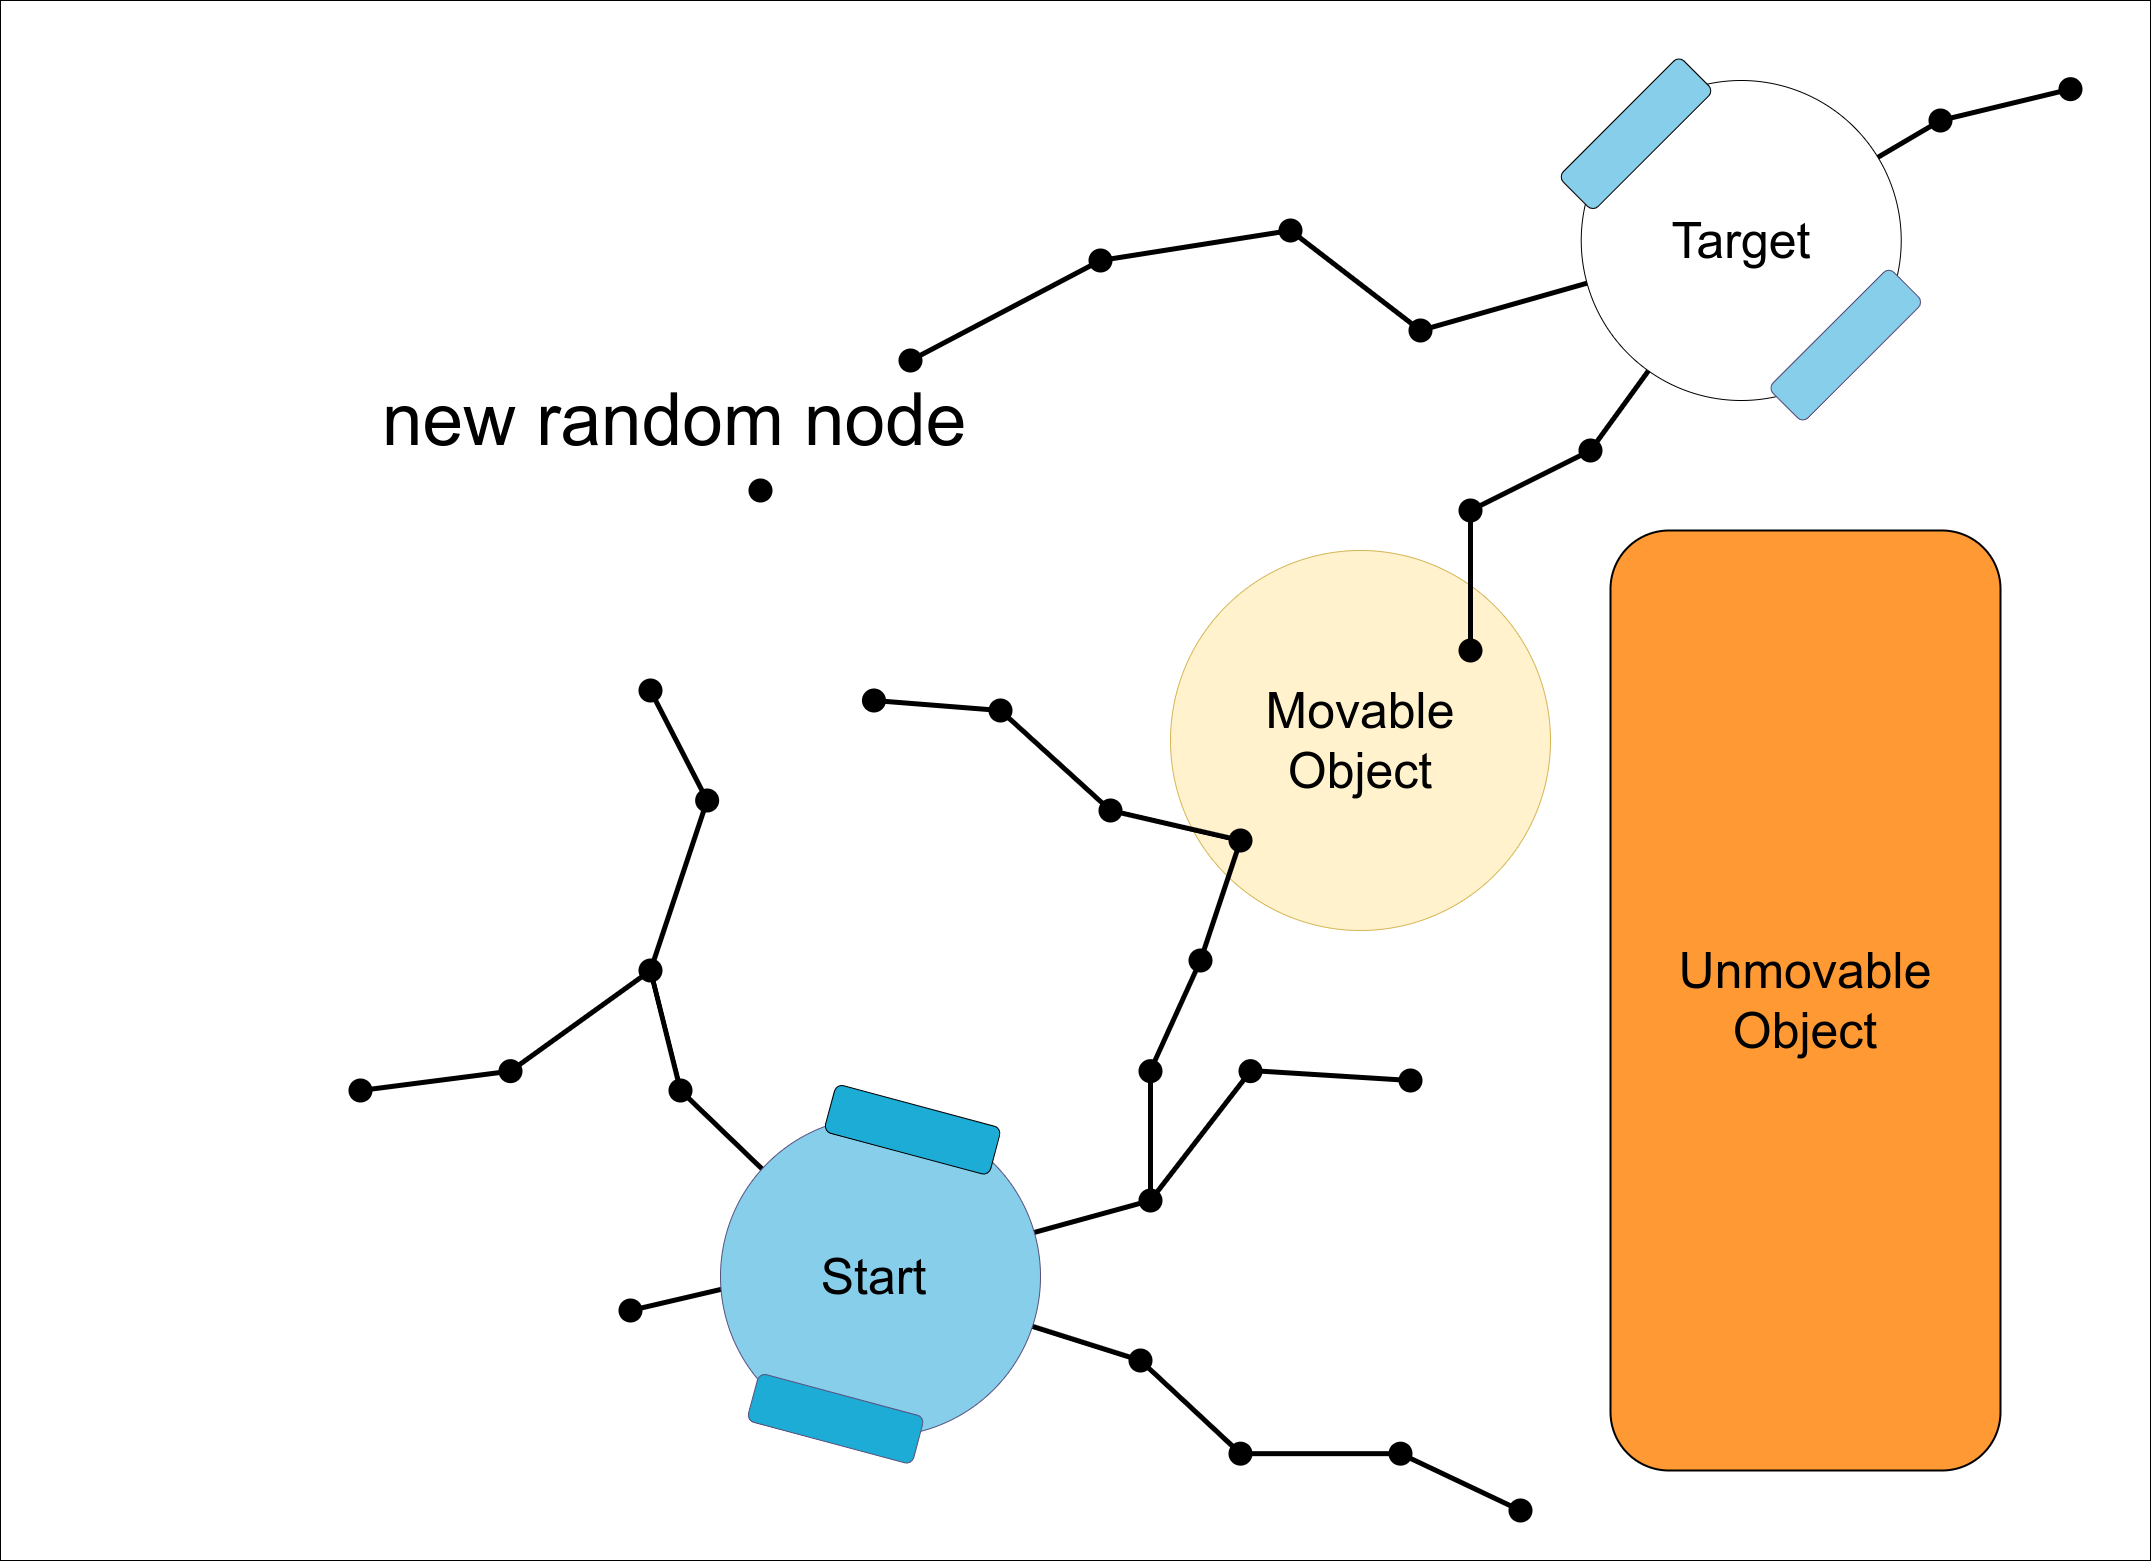
\includegraphics[width=0.93\textwidth, cfbox=my_light_blue 5pt 0pt]{figures/required_background/mp/2mp_new_rand_sample.drawio.png}
    \caption{A new random node is generated.\newline\newline}
    \end{subfigure}
    \begin{subfigure}{.49\textwidth}
    \centering
    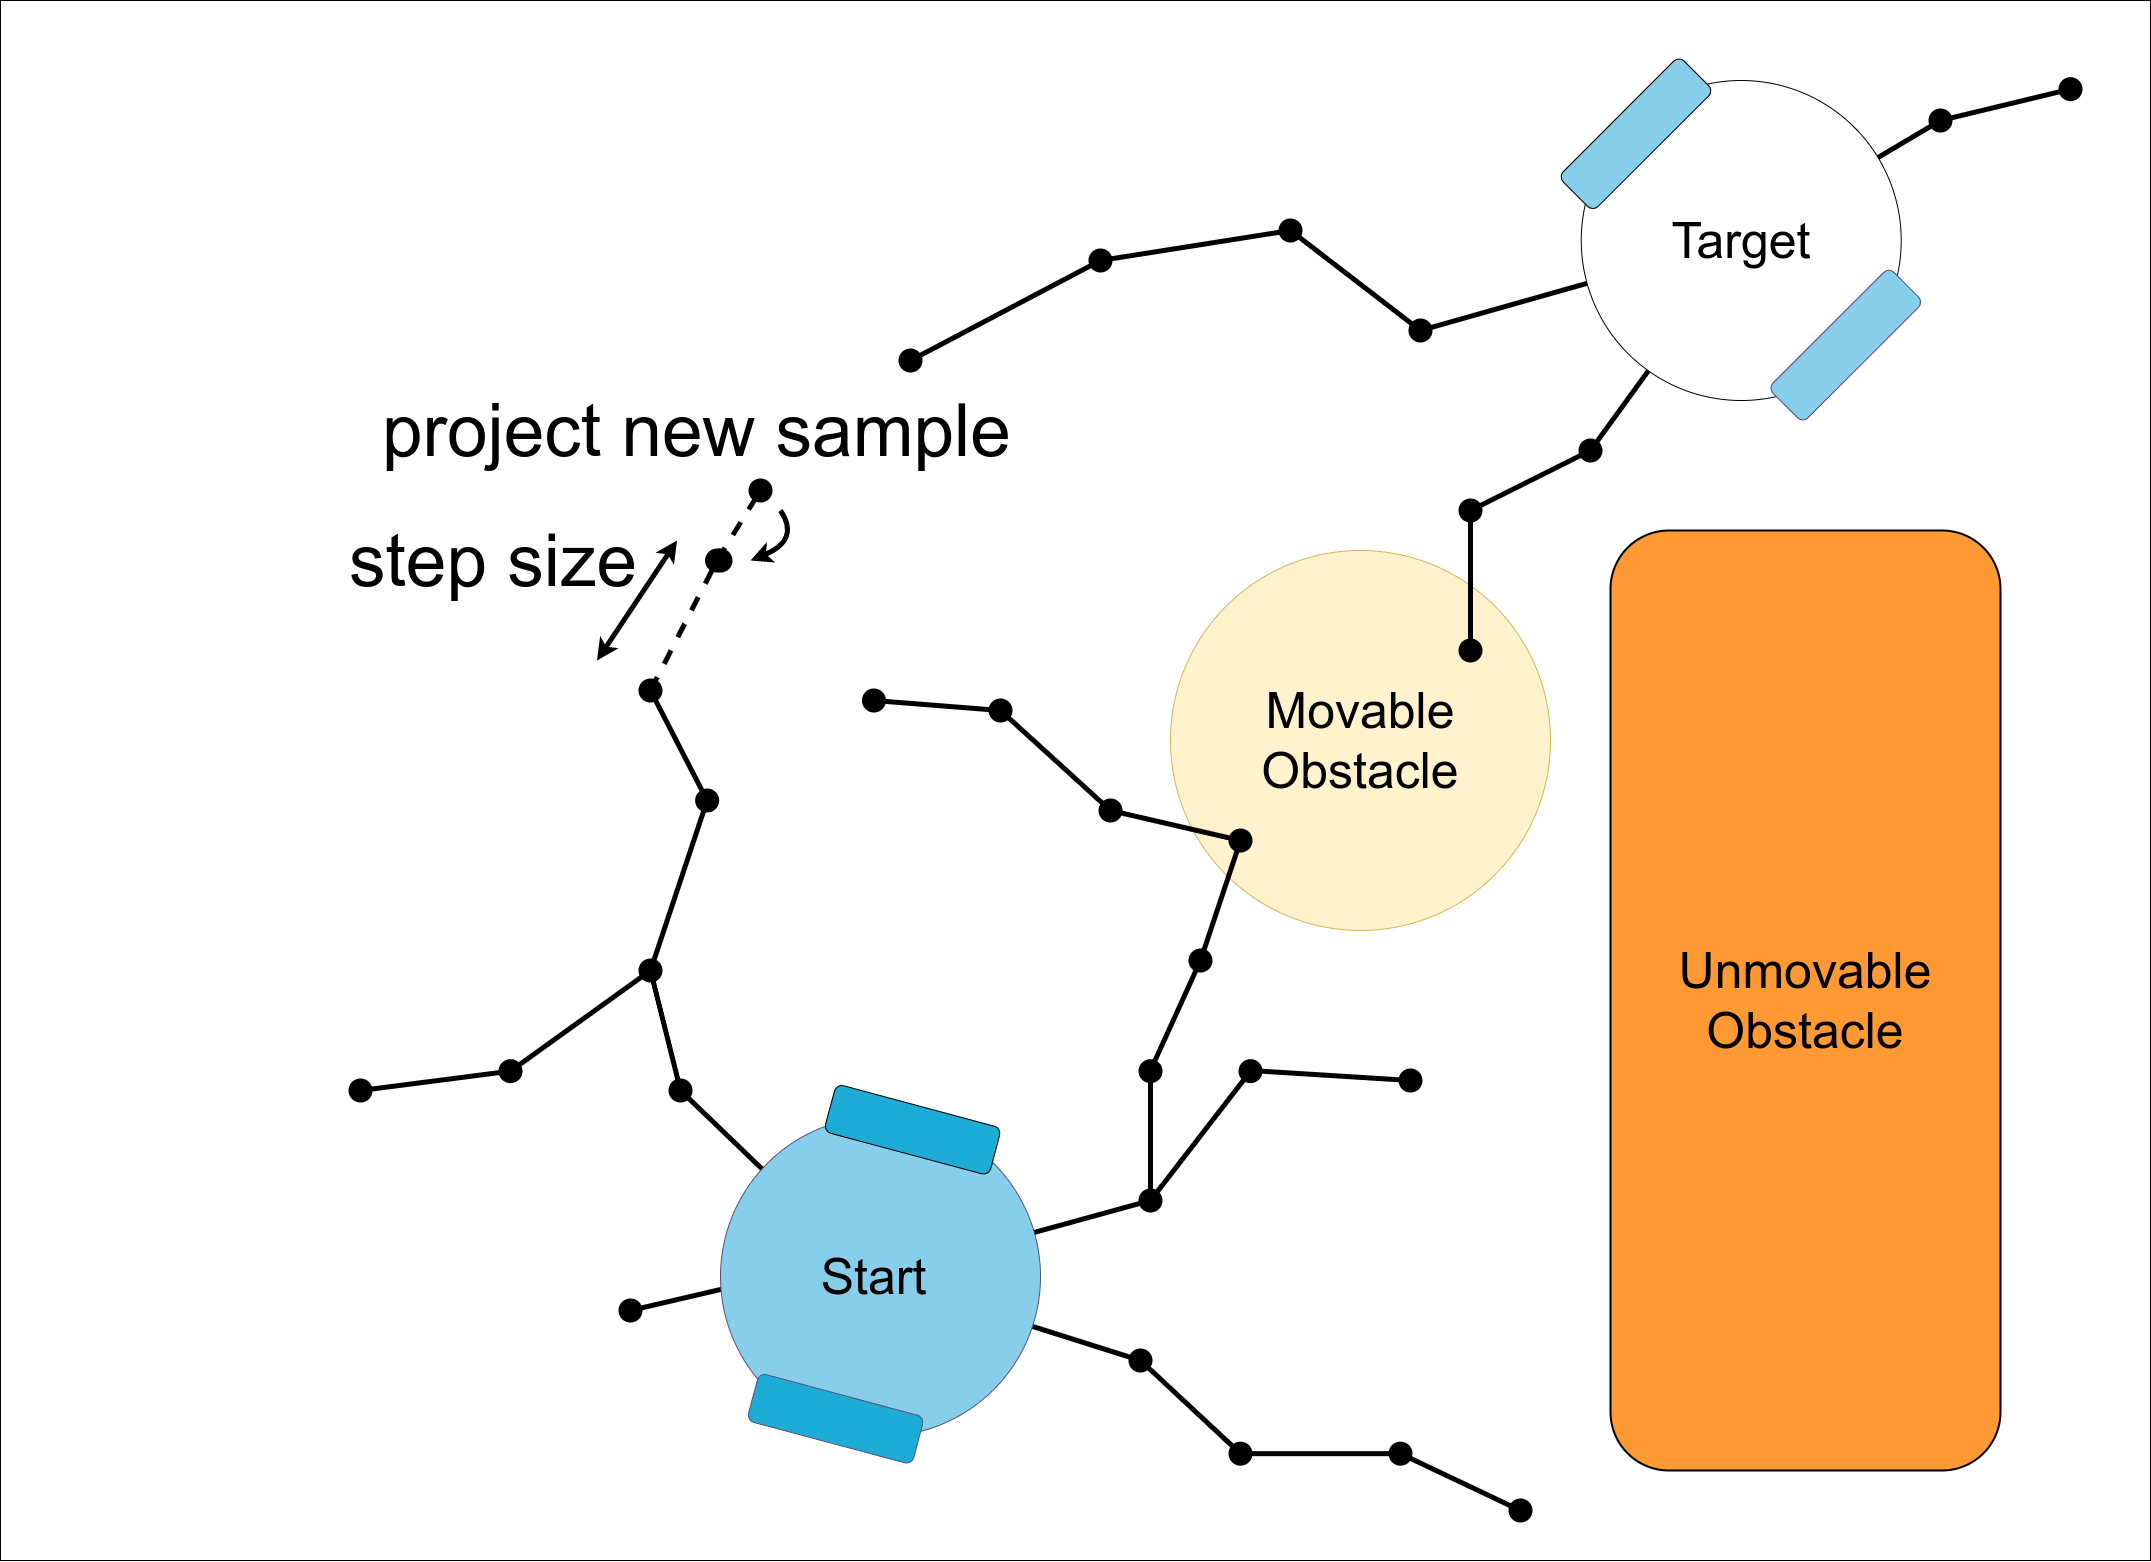
\includegraphics[width=0.93\textwidth, cfbox=my_light_blue 5pt 0pt]{figures/required_background/mp/3mp_project_sample.drawio.png}
    \caption{The new node is projected toward the\\closest node, that becomes its parent node.\bs}%
    \label{subfig:mp_step_size}
    \end{subfigure}

    \caption{Create new node and connect to parent node.}
    \label{fig:motion_planner_adding_one_node_one}
\end{figure}

The new node resides in free space and should now be added to either the start- or target connectivity graph. Adding the new node to either connectivity graph is an operation that creates a new edge between the new node and a to be determined parent node. The operation requires three functions, first a $\mathit{NearestSet}(x, V)$ function that returns set of nearest nodes from $x$ in $V$ that lie in the search space. The parent node is selected from the set of nearest nodes, from this set the node that results in the lowest $\mathit{Cost_{toInit}}$ is sought, defined as:\bs

\[\mathit{Cost_{toInit}} = \mathit{CostToInit(\gls{nodeMP}_{near})} + \mathit{Distance}(\gls{nodeMP}_{near}, \gls{nodeMP}_{new})\]

The $\mathit{Cost_{toInit}}$ is proportional to the path length from a node toward the initial node in the connectivity graph. It can be seen as half of the $\mathit{Cost_{path}}$ that will be later defined as te cost for the entire path from starting- to target node. The second and third functions are the $\mathit{Distance}(x, x')$ function that returns the distance between node $x$ and $x'$, and a $\mathit{CostToInit}(x)$ function that finds the total cost from $x$ to the initial node.\bs

% TWO
\begin{algorithm}[H]
\caption{Pseudocode to find and connect new node to parent node.}%
\label{pseudocode:proposed_rrt_star_two}
\begin{algorithmic}[1]
\hspace{-0.9cm}\colorbox{my_yellow}{\parbox{\linewidth}{%
    \State $X_\mathit{near} \leftarrow \mathit{NearestSet(\gls{nodeMP}_{new}, \gls{nodesMP})}$
    \For{$\gls{nodeMP}_\mathit{near} \in X_\mathit{near}$}
    \State $\mathit{Cost_{temp}} \leftarrow \mathit{CostToInit(\gls{nodeMP}_{near}) + Distance(\gls{nodeMP}_{near}, \gls{nodeMP}_{new})}$
    \If{$\mathit{Cost_{temp}}  < \mathit{Cost_{toInitMin}}$}
    \State $\mathit{Cost_{toInitMin}} \leftarrow \mathit{Cost_{temp}}$
    \State $\gls{nodeMP}_\mathit{minCost} \leftarrow \gls{nodeMP}_\mathit{near}$
        \EndIf
    \EndFor
    \If{$\mathit{Cost_{toInitMin}} == \infty$}
        \State Continue
    \Else
    \State $\gls{nodesMP}.add(\gls{nodeMP}_\mathit{new})$
    \State $E.\mathit{add}(\gls{nodeMP}_\mathit{minCost}, \gls{nodeMP}_\mathit{new})$
    \EndIf
}}
\end{algorithmic}
\end{algorithm}

\begin{figure}[H]
    \centering
    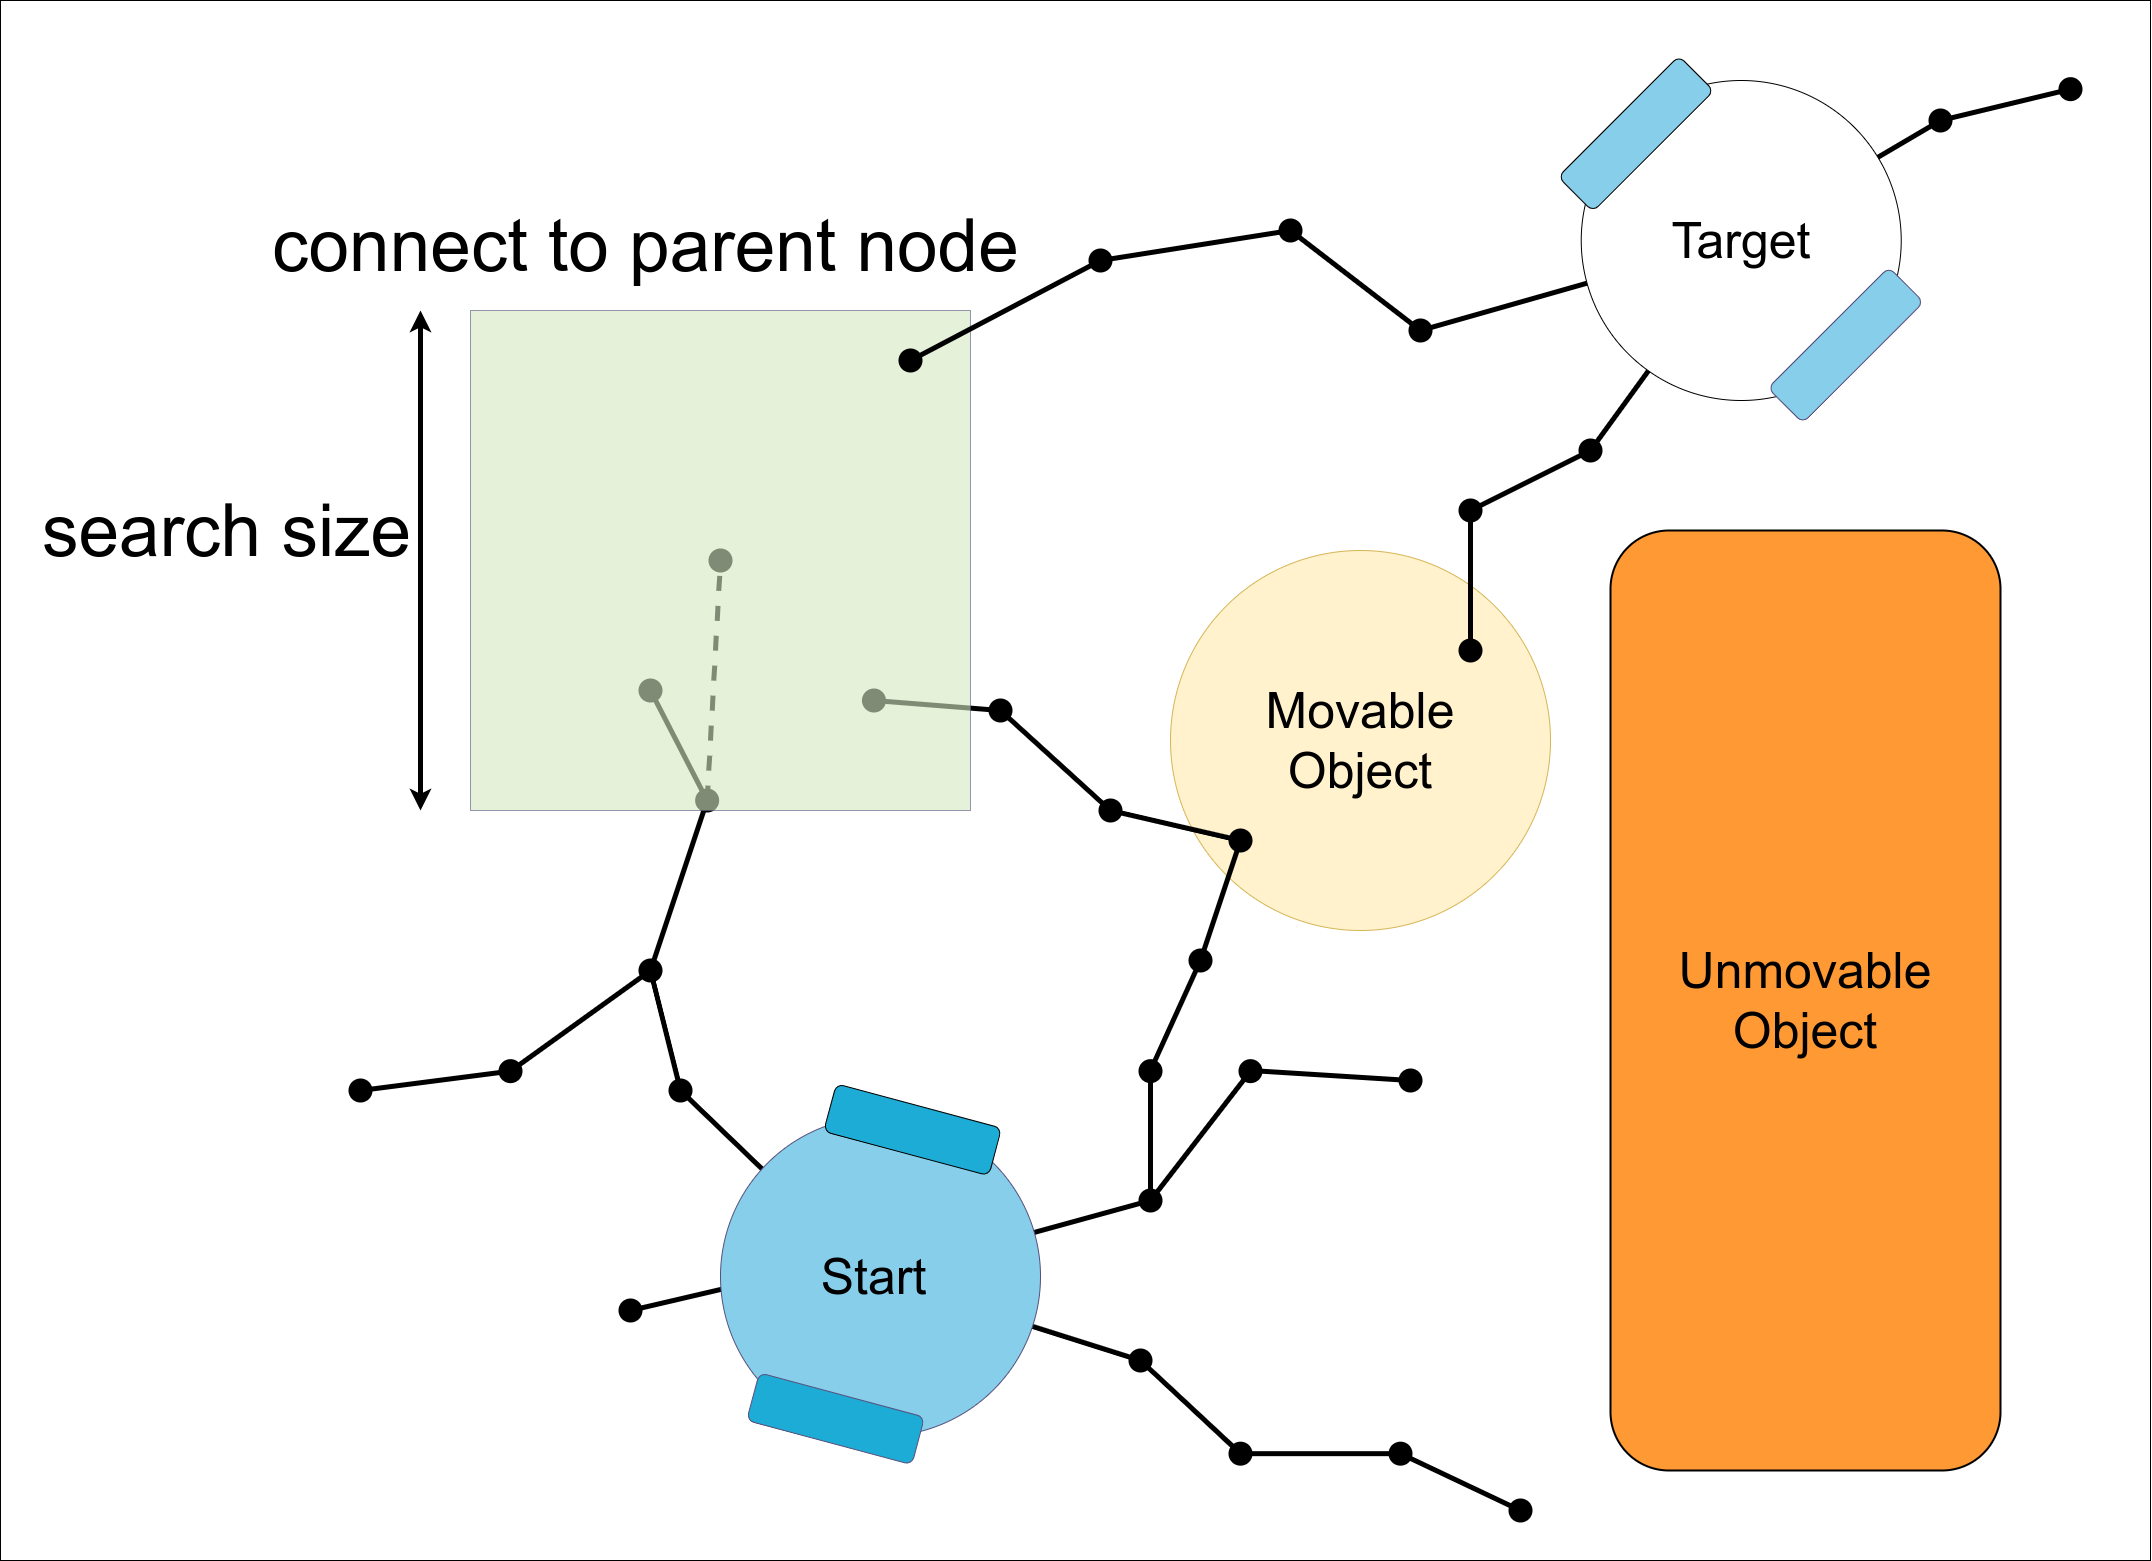
\includegraphics[width=0.5\textwidth, cfbox=my_yellow 5pt 0pt]{figures/required_background/mp/4mp_connect_to_tree.drawio.png}
    \caption{Connect new node to parent node that results in the lower $\mathit{Cost_{toInit}}$.}%
    \label{fig:motion_planner_adding_one_node_two}
\end{figure}

The new node is connected to a parent node as can be seen in \Cref{fig:motion_planner_adding_one_node_tree}. A final step remains to be done, connecting the two trees or rewiring. For this step the $\mathit{InSameTree}(x, x')$ indicates if both $x$ and $x'$ are or are not in the same tree. For every node in the set of nearest nodes that is in the same tree as the new node, it is validated if rewiring would result in a lower $\mathit{Cost_{toInit}}$ for that node. The rewire procedure changes the parent node by removing and adding an edge, rewiring can be visually seen in \Cref{subfig:mp_rewire}. The node in the set of nearest nodes that are in the other three that results in the lowerst $\mathit{Cost_{path}}$ is connected to the new node. Thereby creating a path from start node to target node, the path is added to the set of paths with corresponding $\mathit{Cost}_\mathit{path}$, defined as:\bs

\[\mathit{Cost_{path}} = \mathit{CostToInit(\gls{nodeMP}_{new})} + \mathit{Distance}(\gls{nodeMP}_{new}, \gls{nodeMP}_{other\_tree}) +\mathit{CostToInit(\gls{nodeMP}_{other\_tree})} \]

% THREE
\begin{algorithm}[H]
\caption{Pseudocode to check if the newly added node can lower cost for nearby nodes with the rewire procedure, and if both trees can be connected, yielding a path.}%
\label{pseudocode:proposed_rrt_star_three}
\begin{algorithmic}[1]
\hspace{-0.9cm}\colorbox{my_green}{\parbox{\linewidth}{%
    \State $\mathit{Cost_{pathMin}} \leftarrow +\infty$
    \For{$\gls{nodeMP}_\mathit{near} \in X_{near}$}
    \If{$\mathit{InSameTree(\gls{nodeMP}_{near}, \gls{nodeMP}_{new})}$}
    \If{$\mathit{CostToInit(\gls{nodeMP}_{new}) + Distance(\gls{nodeMP}_{new}, \gls{nodeMP}_{near})} < \mathit{CostToInit(\gls{nodeMP}_{near}})$}
    \State $\mathit{E.rewire(\gls{nodeMP}_{near}, \gls{nodeMP}_{new})}$
        \EndIf
      \Else \algorithmiccomment{Add lowest cost path to the list of paths}
      \State $\mathit{Cost_{temp} \leftarrow CostToInit(\gls{nodeMP}_{new}) + Distance(\gls{nodeMP}_{new}, \gls{nodeMP}_{near})} + \mathit{CostToInit(\gls{nodeMP}_{near})}$
          \If{$\mathit{Cost_{temp}  < Cost_{pathMin}}$}
          \State $\mathit{Cost_{pathMin} \leftarrow \mathit{Cost}_{temp}}$
          \State $\mathit{\gls{nodeMP}_{pathMin} \leftarrow \gls{nodeMP}_{near}}$
          \EndIf
      \EndIf
      \If{$\mathit{Cost_{pathMin}} == \infty$}
          \State Continue
      \Else
      \State $\mathit{P.addPath(\gls{nodeMP}_{new}, \gls{nodeMP}_{pathMin}, Cost_{pathMin})}$
      \EndIf
    \EndFor
}}
\end{algorithmic}
\end{algorithm}

When the start connectivity tree is close enough (inside the search size of a newly added node) to the target connectivity tree, a path from start to target is found. The  
Increasing the search size improves the choice of the parent node and improves cost due to rewiring, but it also exponentially increases computation time.


\begin{figure}[H]
    \centering
    \begin{subfigure}{.49\textwidth}
    \centering
    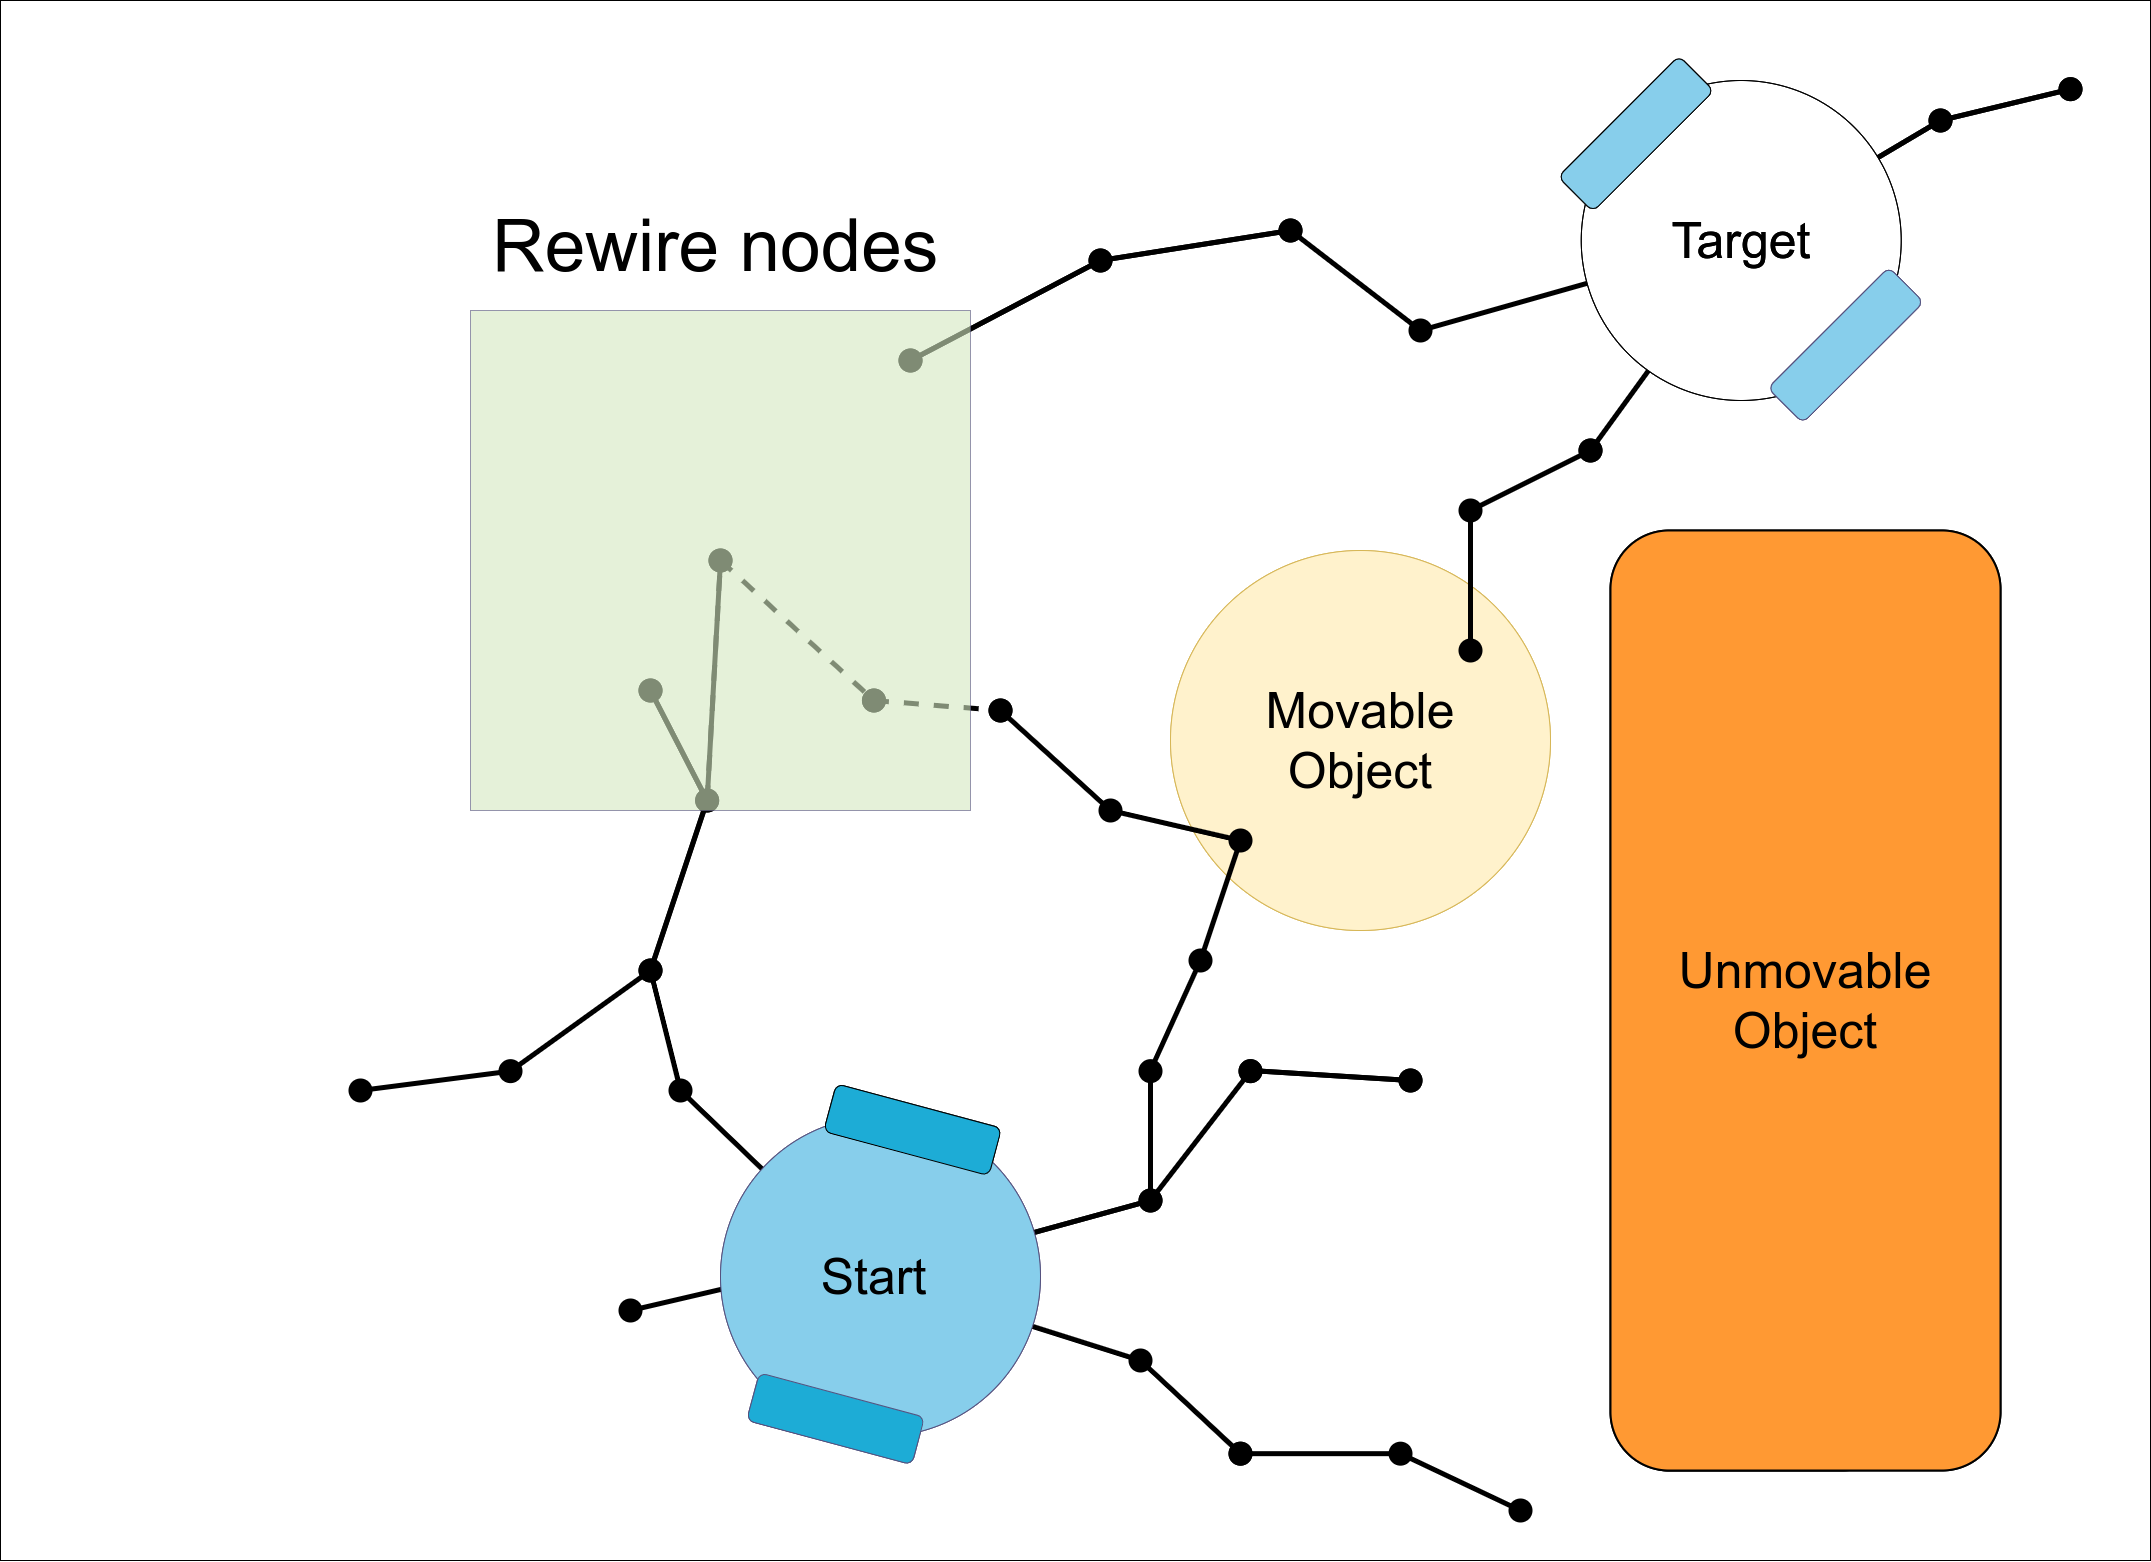
\includegraphics[width=0.93\textwidth, cfbox=my_green 5pt 0pt]{figures/required_background/mp/5mp_rewire.drawio.png}
    \caption{Rewire a node for which the cost can\\be lowered by removing and adding an edge.}%
    \label{subfig:mp_rewire}
    \end{subfigure}
    \begin{subfigure}{.49\textwidth}
    \centering
    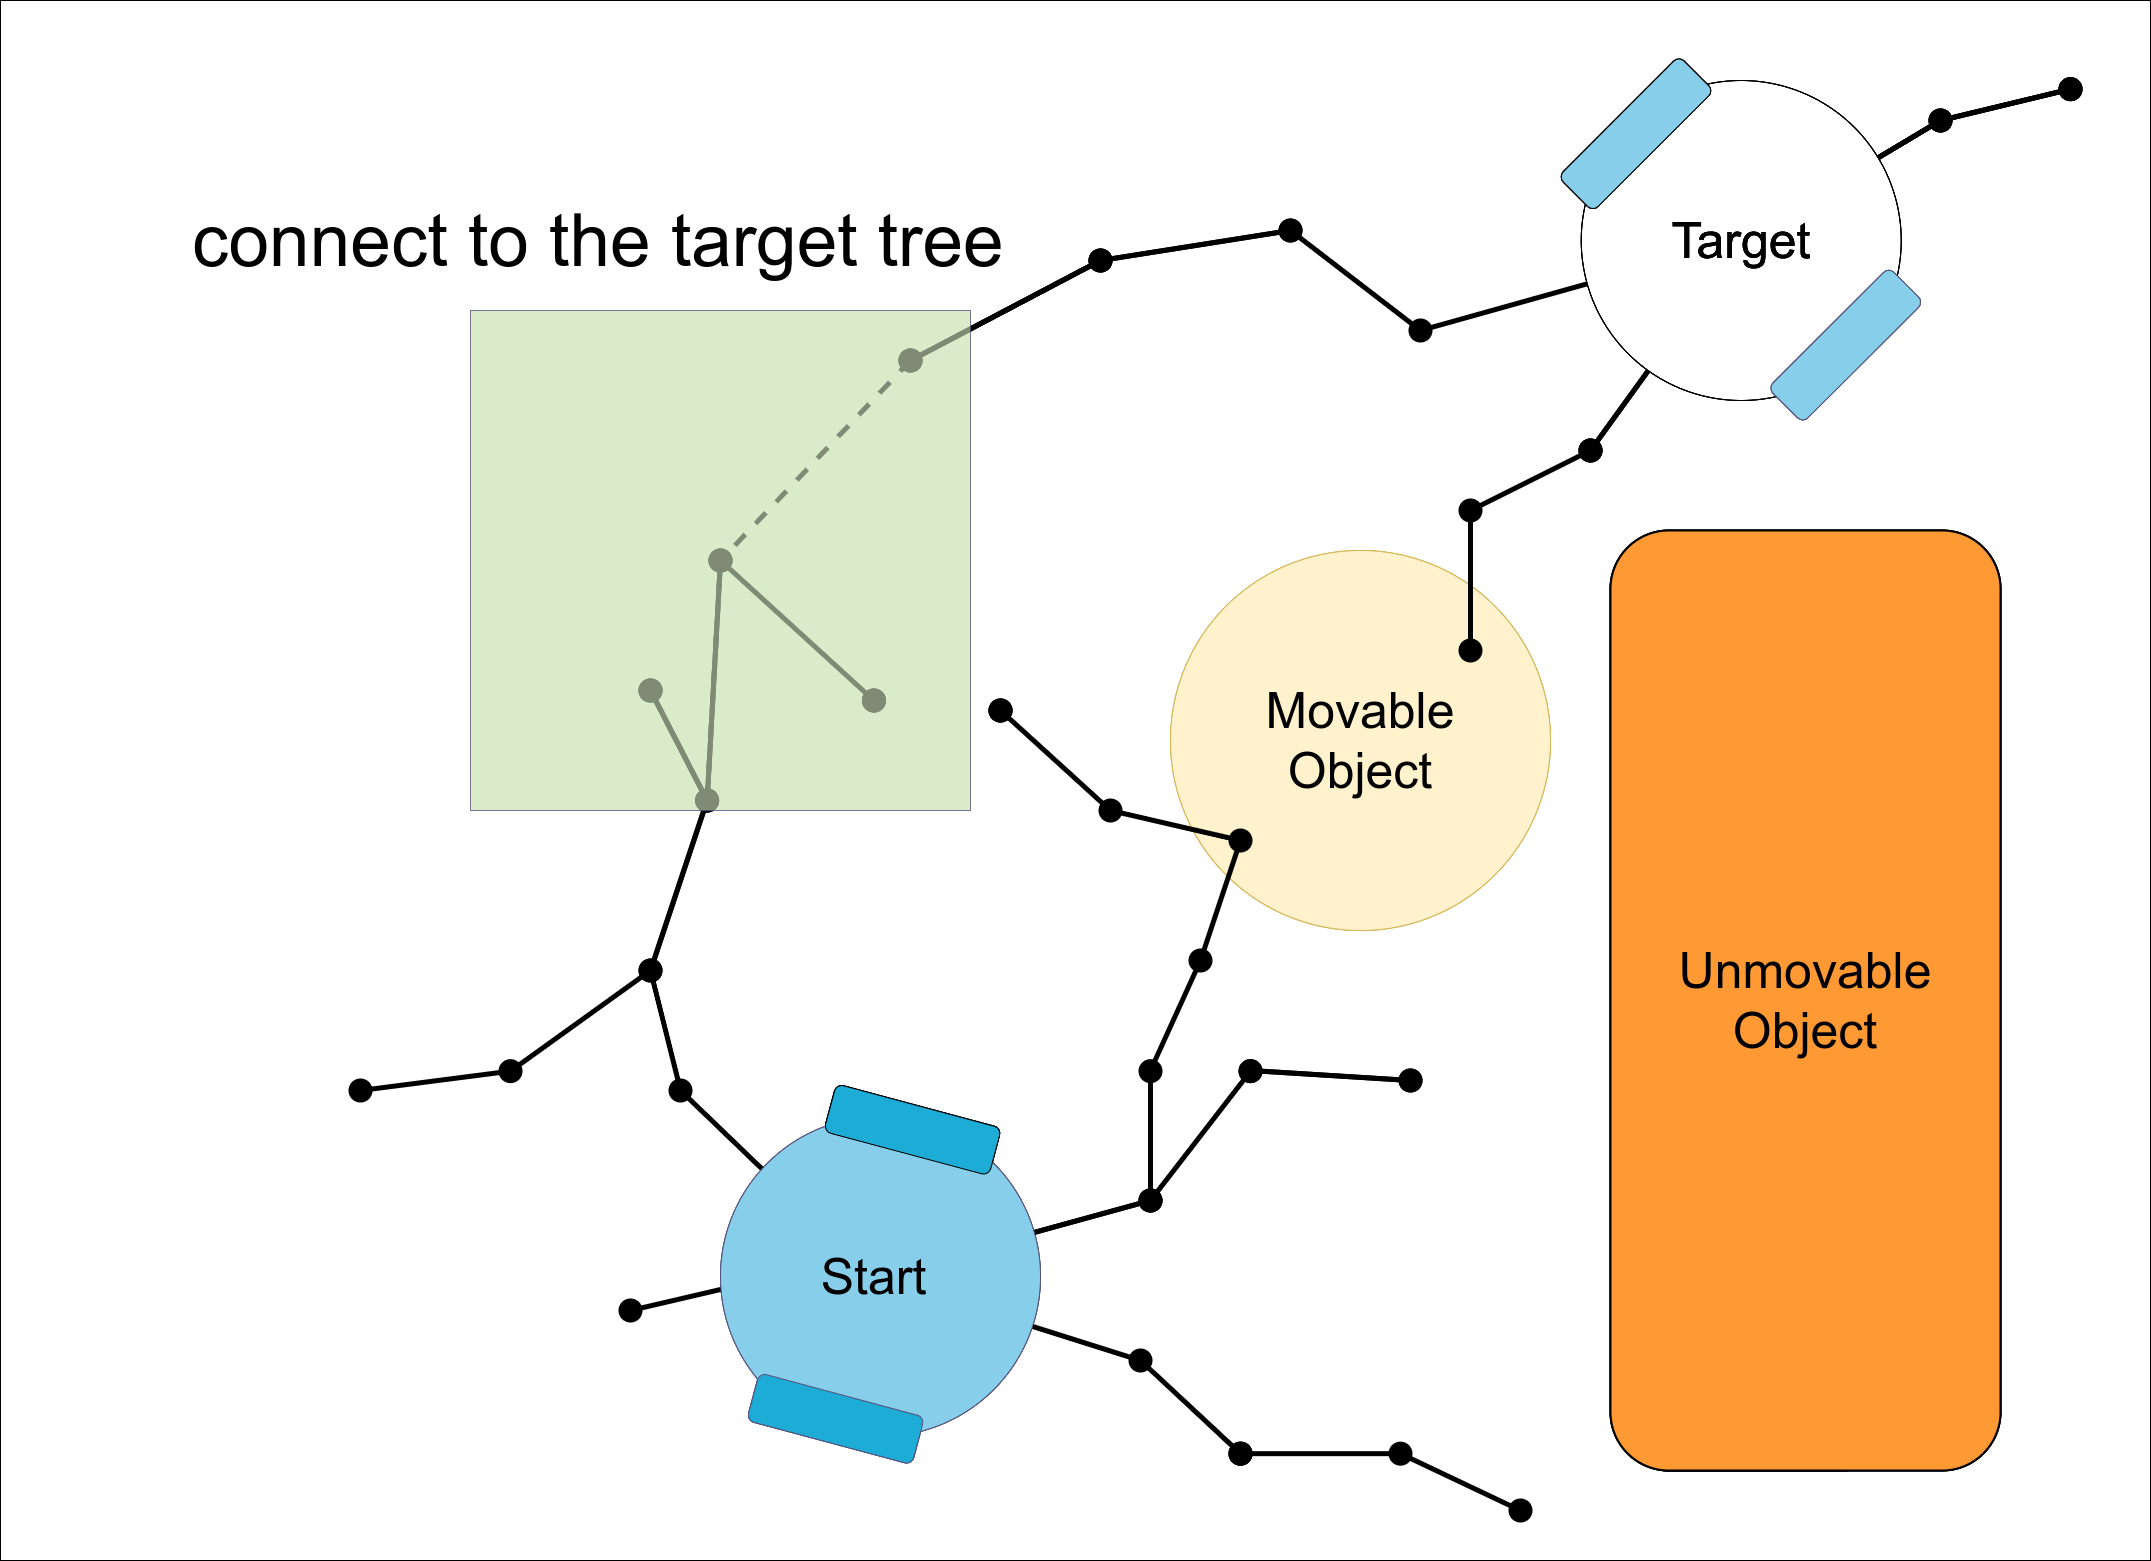
\includegraphics[width=0.93\textwidth, cfbox=my_green 5pt 0pt]{figures/required_background/mp/6mp_search_other_tree.drawio.png}
    \caption{Connect start- to target connectivity tree.\bs}
    \end{subfigure}
    \caption{Check if the newly added node can lower cost for nearby nodes and connect the start- to the target tree.}
    \label{fig:motion_planner_adding_one_node_tree}
\end{figure}

\begin{figure}[H]
    \centering
    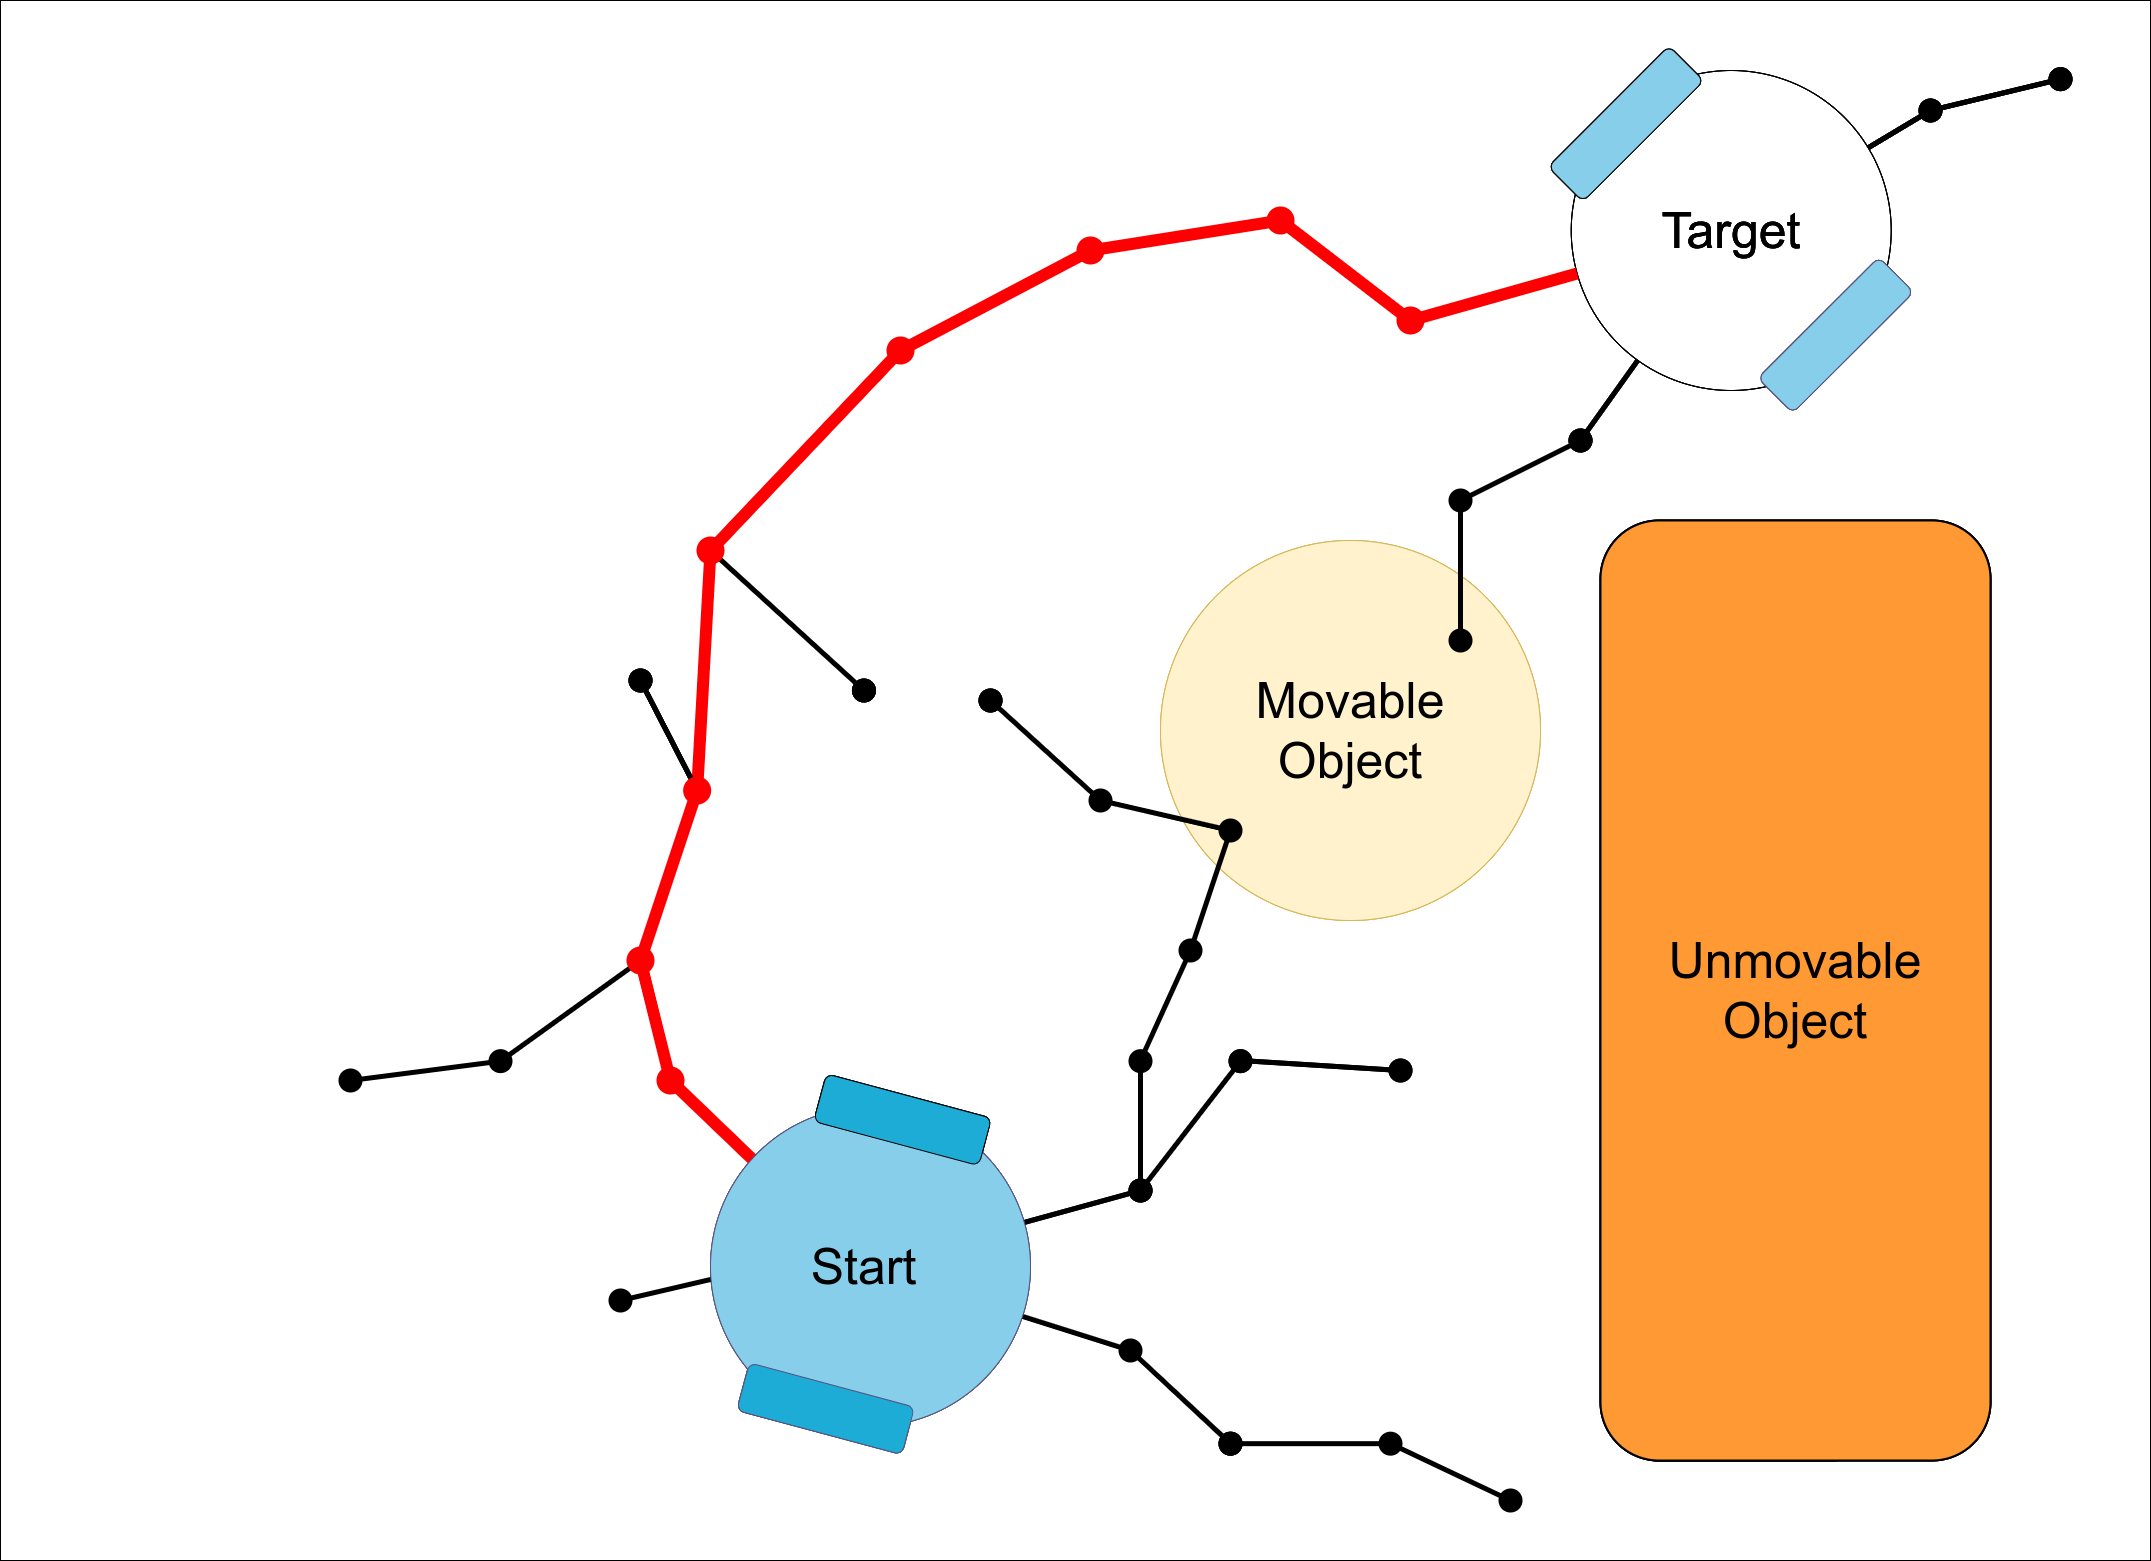
\includegraphics[width=0.5\textwidth, cfbox=my_grey 5pt 0pt]{figures/required_background/mp/7mp_path_found.drawio.png}
    \caption{Path planner that found a path from start= to target node marked in red.}
    \label{fig:motion_planner_adding_one_node_final}
\end{figure}

The existing path planner has now been discussed, the following table summarized the variables and functions. In the upcoming chapter, the path planner is extended to detect blocking paths.\bs
\todo{TotalPathCost is not yet defined, but overwritten in next chapter? define it!}

\noindent
\begin{table}[H]
\centering
  \begin{tabular}%
  {>{\raggedright\arraybackslash}p{0.22\textwidth}%
   >{\raggedright\arraybackslash}p{0.68\textwidth}}
   $x$:& A node consisting of the following tuple: $ \left\langle \gls{c}, \mathit{cost\_to\_source}, \mathit{key}, \mathit{prev\_node\_key}, \mathit{in\_tree} \right\rangle$ where \gls{c} a point in configuration space, \textit{cost\_to\_source} the cost toward the source node $x_{init}$, \textit{key} a unique key for the node, \textit{prev\_node\_key} they parent key to which the node is directly connected, \textit{in\_tree} an indicator that the node is connected to the \textit{start-} or \textit{target} connectivity tree.\\
   $x_{init}$:& The two initial nodes, $x_{\mathit{start}}$ and $x_{\mathit{target}}$\\
  \textit{NotReachStop}:& True if the stopping criteria are not reached\\
  $\mathit{Sample_{random}}$:& Creates a random node in free-, movable- or unknown space\\
  $\mathit{Nearest}(x, V)$:& Returns the nearest nodes from $x$ in $V$\\
  $\mathit{NearestSet}(x, V)$:& Returns set of nearest nodes from $x$ in $V$\\
  $\mathit{Project}(x, x')$:& Project $x$ toward $x'$\\
  $\mathit{CollisionCheck}(x)$:& Returns true if $x$ is in free space\\
  $\mathit{Distance}(x, x')$:& Returns the distance between node $x$ and $x'$\\
  $\mathit{CostToInit}(x)$:& Find the total cost from $x$ to the initial node\\
    $\mathit{InSameTree}(x, x')$:& Returns true if both $x$ and $x'$ are in the same tree, otherwise return false\\
  \end{tabular}
\caption{The variables and functions employed in the \Cref{pseudocode:proposed_rrt_star_all,pseudocode:proposed_rrt_star_one,pseudocode:proposed_rrt_star_two,pseudocode:proposed_rrt_star_three}.}
\label{table:functions_for_proposed_rrt_star}
\end{table}
